%----------------
%  ÍNDICES
%----------------
\cleardoublepage
\tableofcontents % Prints the main table of contents

\listoffigures % Prints the list of figures

\listoftables % Prints the list of tables

%----------------
%  SIGLAS
%----------------
\cleardoublepage
\begin{abbreviations}{ll} % Include a list of abbreviations (a table of two columns)

\textbf{AEAT} & \textbf{A}gencia \textbf{E}statal de \textbf{A}dministración \textbf{T}ributaria\\
\textbf{ANPR} & \textbf{A}utomatic \textbf{N}umber-\textbf{P}late \textbf{R}ecognition\\
\textbf{API} & \textbf{A}pplication \textbf{P}rogramming \textbf{I}nterface\\
\textbf{AP} & \textbf{A}ffinity \textbf{P}ropagation\\
\textbf{ASC} & \textbf{A}ttributed \textbf{S}pectral \textbf{C}lustering\\
\textbf{AIC} & \textbf{A}kaike \textbf{I}nformation \textbf{C}riterion\\
\textbf{BIC} & \textbf{B}ayesian \textbf{I}nformation \textbf{C}riterion\\
\textbf{CH} & \textbf{C}alinski-\textbf{H}arabasz Score\\
\textbf{DB} & \textbf{D}ata \textbf{B}ase\\
\textbf{DBI} & \textbf{D}avies-\textbf{B}ouldin \textbf{I}ndex\\
\textbf{DGT} & \textbf{D}irección \textbf{G}eneral de \textbf{T}ráfico\\
\textbf{DTW} & \textbf{D}ynamic \textbf{T}ime \textbf{W}arping\\
\textbf{EM} & \textbf{E}xpectation \textbf{M}aximization\\
\textbf{GPS} & \textbf{G}lobal \textbf{P}ositioning \textbf{S}ystem\\
\textbf{IC} & \textbf{I}nformation \textbf{C}riterion\\
\textbf{INE} & \textbf{I}nstituto \textbf{N}acional de \textbf{E}stadística\\
\textbf{IO} & \textbf{I}ndoor-\textbf{O}utdoor\\
\textbf{IP} & \textbf{I}nternet \textbf{P}rotocol\\
\textbf{IoT} & \textbf{I}nternet \textbf{O}f \textbf{T}hings\\
\textbf{LPR} & \textbf{L}icense \textbf{P}late \textbf{R}ecognition\\
\textbf{MAD} & \textbf{M}edian \textbf{A}bsolute \textbf{D}eviation\\
\textbf{ML} & \textbf{M}achine \textbf{L}earning\\
\textbf{MT} & \textbf{M}aster's \textbf{T}hesis\\
\textbf{PCA} & \textbf{P}rincipal \textbf{C}omponent \textbf{A}nalysis\\
\textbf{SC} & \textbf{S}ilhouette \textbf{C}oefficient\\
\textbf{SGTM} & \textbf{S}ecretaría \textbf{G}eneral de \textbf{T}ransportes y \textbf{M}ovilidad\\
\textbf{SSB} & \textbf{S}um of \textbf{S}quared \textbf{B}etween\\
\textbf{SSW} & \textbf{S}um of \textbf{S}quared \textbf{Within}\\ 

\end{abbreviations}

\begin{comment}
%----------------
% CONSTANTES Y DEFINICIONES
%----------------
\cleardoublepage
\begin{constants}{lr@{${}={}$}l} % The list of physical constants is a three column table

% The \SI{}{} command is provided by the siunitx package, see its documentation for instructions on how to use it

Speed of Light & $c_{0}$ & \SI{2.99792458e8}{\meter\per\second} (exact)\\
%Constant Name & $Symbol$ & $Constant Value$ with units\\

\end{constants}

%----------------
% SÍMBOLOS Y CONCEPTOS
%----------------------------------------------------------------------------------------
\cleardoublepage
\begin{symbols}{lll} % Include a list of Symbols (a three column table)

$a$ & distance & \si{\meter} \\
$P$ & power & \si{\watt} (\si{\joule\per\second}) \\
%Symbol & Name & Unit \\

\addlinespace % Gap to separate the Roman symbols from the Greek

$\omega$ & angular frequency & \si{\radian} \\

\end{symbols}
\end{comment}

%----------------
% CONTENIDO DEL TFM
%----------------
\cleardoublepage
\mainmatter % Begin numeric (1,2,3...) page numbering
\pagestyle{thesis} % Return the page headers back to the "thesis" style

% Include the chapters of the thesis as separate files from the Chapters folder
% Uncomment the lines as you write the chapters

\chapter{Introduction}

Currently, there are 13.4 billion Internet of Things (IoT) devices. Statista predicts that this figure will increase to 29.4 billion by 2030\footnote{\url{https://www.statista.com/statistics/1183457/iot-connected-devices-worldwide/}}. These devices form an interconnected network that produces extensive data in numerous social domains. Access to a large volume of data collected by various sensors makes it possible to supervise and manage different aspects of society, including healthcare, evacuation systems, smart environments, and transportation.~\cite{atzori2010internet,bermudez2018analysing,garcia2022machine, centelles2019lora}. Extracting and combining information from multiple sources, not only sensor data, but also information stored on the Internet, can lead to a better understanding of the problem to be solved, such as healthcare or vehicle mobility. For example, traffic in cities is partially dependent on local holidays. These multi-source data have resulted in the growth of some research fields, such as information fusion, intelligent environments, and ubiquitous computing. The insights from analyzing these multisource datasets can be applied to real-world problems such as tourism management, economics, and financial information systems~\cite{haughton2004sustainable}.

The number of studies with smart city data has grown exponentially in recent years. The most important cities have deployed sensor networks and IoT platforms. The data obtained by these sensors have led to numerous studies in several areas, such as traffic behavior \cite{mondal2019identifying,lin2019application,peixoto2021traffic,ning2019vehicular}. However, most solutions that try to cluster different traffic behavior do not have additional information, such as the residence of vehicle owners, to provide additional insight into the explainability of the clusters. Furthermore, this smart city trend has yet to reach small villages, and the solutions found for large cities do not always apply directly to small villages. For example, solutions monitoring traffic behavior in large cities with numerous streets and several traffic lines in some avenues do not extrapolate to villages with 6 or 7 mostly pedestrian streets and only one road with one line in each direction. Additionally, even if we try to add some explanation to the behavioral cluster in smart villages, the residency of vehicle owners is not straightforward. Due to the recent movement on moving from cities to villages and retrying or spending long periods on second residences, the actual residence information is fuzzy in rural villages.

This work proposes a clustering based on vehicle behavior in small villages, with information from license plate recognition (LPR) devices and owners' residences, among others. We applied the study directly to each individual (vehicles) and defined their spatio-temporal behavior based on their spatial frequencies of visitation. To that end, we fused several datasets and calculated new valuable variables such as the time spent in the area; total distance traveled there, etc. We study the popularly used clustering algorithms to draw conclusions on which of them performs better on the problem under consideration. In particular, we used a pipeline to analyze the particularities of the data through several visualization tools, and we explained, based on the data, the optimal normalization and clustering algorithm that best groups the different behaviors of the vehicles. We will focus on the importance of selecting the optimal normalization algorithm and its influence on the results. Additionally, we analyzed the results with residential information and determined the variables that most influence each cluster. With this information, we explained the behavior pattern of each cluster. Our pipeline comprises eight steps: data collection, cleaning, fusion, normalization, dimensionality reduction, clustering, evaluation, and visualization. Finally, we applied the proposed pipeline to a touristic rural region, with the problems mentioned above of a single small road and the lack of reliable residency information.

The findings of our research hold significant implications for policymakers, particularly in managing tourism flows in smart cities and villages. By integrating multiple data sources and employing appropriate clustering and normalization algorithms, our proposed pipeline enables a comprehensive analysis of mobility patterns. The enriched dataset, with its valuable insights into different patterns, can inform policymakers about the dynamics of tourism flows in specific areas. This knowledge is crucial for managing and optimizing transportation systems, infrastructure development, and resource allocation to accommodate the needs of both residents and visitors. By understanding the traffic patterns among residents and tourists in a rural touristic area, policymakers can devise targeted strategies to enhance visitor experiences, reduce congestion, and mitigate the environmental impact associated with tourism activities. The data analysts and policymakers can utilize our research to select suitable algorithms and gain a deeper understanding of mobility patterns, thus facilitating evidence-based decision-making and the effective management of tourism flows in environmentally sensitive areas.

\section{Motivation}

In conducting a literature review, I observed a significant gap in the analysis of smart villages and car behavior within these environments, compared to the abundance of articles focused on smart cities. In addition, there was limited exploration of normalization techniques in this context. This realization sparked a personal interest and desire to tackle the challenge of working with sensors and creating a comprehensive database from a simple one constructed from timestamps and license plate data.

Given my background, I was able to combine different fields of expertise, combining my previous knowledge in computer science with those acquired during my master's degree, such as business intelligence, data visualization and information extraction for policymakers. During my degree, I did a simple internship on clustering analysis, and dealing with the topic of unsupervised learning in the master's degree, aroused even more my interest to go deeper into this topic.

As an additional motivation, the completion of this Master's Thesis (MT) is also linked to Smart Poqueira\footnote{\url{https://wpd.ugr.es/~smartpoqueira/}} a subproject included in the project "Thematic Center on Mountain Ecosystem \& Remote sensing, Deep learning-AI e-Services" (LifeWatch-2019-10-UGR-01), linked to the analysis of different aspects related to the conservation of the Sierra Nevada National Park through advanced digital systems. The project has been co-funded by the Ministry of Science and Innovation through the ERDF funds of the Pluriregional Operational Program of Spain 2014-2020 (POPE), LifeWatch-ERIC action line, with the co-funding of the Provincial Council of Granada and the University of Granada. The heads of the Provincial Council and the University of Granada have pointed out that this commitment to the use of digital technology and innovation will make it possible to efficiently manage numerous data on the behavior of its visitors and, thus, implement solutions that improve the quality and sustainability of the visits received.

In addition to the connection with the Smart Poqueira Project, this MT is closely related to several subjects learned in the Master's program, providing a solid foundation and relevant knowledge for its development. The following are some of the areas from the master's degree courses that have a strong relationship with this dissertation:

\begin{itemize}
\item \textbf{Analysis and Inference in Business Processes}: This course has provided me with a background in machine learning techniques and validation metrics. By leveraging this knowledge, I have been able to develop intelligent systems that extract relevant information and patterns for decision-making in the field of sustainable tourism. 

\item \textbf{Business Intelligence}: Data analysis related to business strategy is a key element in implementing sustainable tourism solutions. In this subject, I have improved my skills in collecting, analyzing, and visualizing data, enabling me to make well-informed decisions for tourism management in the region of Alpujarra. 

\item \textbf{Data Bases for Business Processes}: Effective management of the data collected is crucial to the success of the project. By studying this subject, I have acquired the knowledge necessary to design and ensure the integrity and usefulness of the information collected.

\item \textbf{Big Data and Sustainability}: My understanding of big data and its implications for sustainability in the tourism industry was fostered through the subject of \textbf{Introduction to Management and Technologies in Business Processes}. Efficient management of collected data, its analysis, and the generation of insights from it will be key elements in making informed decisions and developing strategies that foster sustainability in the tourism sector.

\item \textbf{Project Management and Planing}: Effective communication and planning are essential for successful project execution. In this course, I have learned how to establish clear lines of communication with suppliers and stakeholders. In addition, this subject has given me project management techniques that support the design of project requirements and timelines essential in project development.

\item \textbf{Business Strategy and Internationalization in Technologically Advanced Environments}: In this course, I have learned that, today, organizations and businesses face a rapidly changing and highly competitive global environment. Policymakers and business owners must be agile, flexible and be able to obtain the necessary information for strategic decision-making, which facilitates higher levels of current and future competitiveness. The integration of technologies into business processes facilitates responsiveness, cost reduction, improved productivity and enhanced services.
\end{itemize}

These subjects provide a solid foundation of knowledge and skills that will be directly applied in the development of the MT. Additionally, other competencies from subjects in the program have been developed through teamwork, which has made this work possible. \textbf{Collaborative Systems and Workflow Management} (communication tools with teams and suppliers), \textbf{Dashboards and Multidimensional Systems} (designing KPIs and dashboards linked to the project), and \textbf{Design and Access to Web-Based Information and Content Management} (development of the project's website) have all contributed to the completion of this work. The combination of the connection with the Smart Poqueira project and the relevance to key subjects in the Master's program ensures the significance and applicability of this work, making a significant contribution to the advancement and development of sustainable tourism in Alpujarra.
 
\section{Objectives} \label{objetivos}

% Objetivos se han cumplido en las conclusiones

The objective of this MT is to investigate and analyze traffic behavior in smart villages using license plate recognition (LPR) devices and considering the residence of the owners. The specific objectives are as follows:

\begin{itemize}

\item Study clustering algorithms, machine learning pipelines and normalization algorithms; and the suitability of using specific algorithms for specific data distributions.

\item Review previous works on clustering applied to traffic behavior with LPR.

\item Design and deploy an infrastructure to collect data on vehicle movements in smart villages.

\item Examine, in our use case, the correlation between vehicle behavior and provenance, visitation frequency, length of stay, and seasonality.

\item Evaluate and compare different normalization techniques for preprocessing the collected data.

\item Explore various clustering algorithms and techniques and select the most appropriate ones based on the visualization and explainability of the results.

\item Evaluate the performance of the proposed clustering pipeline and selected clustering and normalization algorithms.
\end{itemize}

By achieving these objectives, this work aims to contribute to the understanding of traffic behavior in smart villages and provide valuable information for the design of effective traffic and tourism management systems and policies in the area.

\section{Thesis Outline}

% Añadir las referencias a las secciones

This chapter has presented the challenges that face the study of traffic in smart villages and the motivation of this dissertation. In Chapter \ref{ch:related_work} related work is summarized. Chapter \ref{ch:fundamentals} presents the theoretical bases discussed throughout the MT, describing the main normalization and clustering algorithms and metrics, as well as the demographic context of the area where the study was conducted. Chapter \ref{ch:methodology} presents the unsupervised learning pipeline, including the sensor's setup and the different sources of information used to construct the dataset. Chapters \ref{ch:results} show the analysis of the results. Finally, Chapter \ref{ch:discussions} concludes the work and Chapter \ref{ch:future} presents the limitations and future work related to the project.
\chapter{Related Work} \label{ch:related_work}

\section{Information Fusion in Smart Cities for Touristic applications}

The concept of information fusion has been applied to the specific problem of tourism flows and smart cities. These approaches use advanced data analysis techniques to combine multiple sources of information, providing valuable insights for developing smart tourism applications in cities and designing sustainable environments. Smart city applications are built on top of data, and data fusion has provided a wide variety of techniques to improve the input data for an application~\cite{lau2019survey}. Examples of these techniques include data association, state estimation, unsupervised machine learning, or statistical inference. For example, combining different tourist information has been used to predict the national tourist flow in Spain with graph neural networks~\cite{saenz2023nation}. The data used in the solution are composed of tourist infrastructure information, such as camping and tourist housing from the data sources OpenStreetMap and the National Institute of Statistics of Spain (INE); reports released by the Spanish Ministry of Transportation (SGTM); and human mobility data including the number of movements between administrative areas per hour extracted from geotagged Twitter data. Most of these applications are focused either on user recommendations or tourist flow, but little attention has been paid to studying the individual behavior of the tourist inside an area (for a detailed survey, see \cite{doborjeh2022artificial, lau2019survey}). 

\section{Clustering and mobility patterns}

The increasing deployment of IoT platforms in smart cities has boosted the proliferation of sensors, including those that monitor traffic. These sensory data allow us to analyze vehicle behavior. The most common works in this area are to analyze mobility patterns in order to improve traffic congestion~\cite{mondal2019identifying,peixoto2021traffic}, and to aggregate vehicles to obtain useful conclusions for urban management~\cite{bolanos2022clustering, lin2019application}. 

To infer mobility patterns from raw data, unsupervised ML is widely adopted. In particular, various industries use clustering algorithms to categorize data into distinct groups based on similarities, differences, and patterns without prior knowledge. Clustering analysis is used to detect behavioral patterns in the field of pedestrian-vehicle mobility, and in the field of indoor-outdoor (IO) positioning systems \cite{mallik2023paving}. Some works use partitional clustering to analyze data. For example, in \cite{yao2021understanding}, the ISODATA clustering algorithm is used to cluster mobility patterns and a decision tree is used to create decision rules between the attributes and the labeling obtained from the clustering. In \cite{sun2021identifying}, they propose a K-Means clustering framework combined with other processes such as dimensionality reduction and feature extraction to classify tourists and locals based on the data generated by each individual's mobile phone signaling data and their movement through the area. Hierarchical clustering \cite{pasupathi2021trend} has also been used to segment time series related to vehicle mobility, with the objective of predicting areas where there is a higher risk of accidents. Other commonly used clustering algorithms are density-based, as they can be adapted to problems where irregular behavior occurs within the population. In \cite{belhadi2021deep}, the authors propose an alternative version of the DBSCAN clustering algorithm to detect collective anomalous human behavior from large amounts of pedestrian data in smart cities. The algorithm uses an iterative search process and aggregation of achievable density data points to form clusters, culminating in a global approach to identify behaviors of particular interest in the population. Density clustering techniques also allow the analysis of movement in areas where some specific transport behaviors are known but where more information about particular groups is desired. In \cite{bai4086627data}, a modified version of DBSCAN (iterative and multi-attribute) was used to cluster the different areas of the port, with the aim of improving organization and resolving port congestion. Algorithms such as GaussianMixture are used to perform segment analysis, where individuals are defined by their movement routines, and the data is related to the frequency and period of stay in different areas. From the movement information provided by smart cards, several papers apply this algorithm to identify market segments based on temporal travel patterns \cite{cats2022unravelling}, define tourist patterns based on frequency and areas where transactions are made \cite{gutierrez2020profiling} or identify changes in functional areas of cities over time \cite{wang2021identifying}.

Few works related to clustering analysis in mobility use LPR cameras as the main source of information \cite{yao2022analysis}. For example, \cite{yao2022analysis} analyze the commuting patterns constructing the spatio-temporal similarity matrix using the dynamic time warping (DTW) algorithm; and afterward, analyze the characteristics of commuting patterns with the density-based spatial clustering of applications with noise (DBSCAN) algorithm. Similarly, \cite{yao2022understanding} analyzes the change in traffic patterns during the pandemic using K-Means. However, none of these works combine LPR data with vehicle provenance nor study the touristic behavior of the vehicle. Likewise, none of them compares the suitability of using different clustering algorithms.

\section{Traffic management and business strategy in villages}

Traffic management and business strategy in rural villages is a crucial topic for the development of rural policies in Europe. The implementation of smart villages presents distinct challenges in both central and peripheral rural areas at the European and national levels. It is necessary to have an integrated vision that takes into account the specific issues, needs and expectations of each country. In this context, Spain finds itself in a situation of dual rural periphery: European and national. There are two paths towards smart villages: the horizontal connection between territories and the businesses that promote diversification \cite{paniagua2020smart}. Depopulated areas are attractive for leisure, work, and retirement. The challenge lies in developing intelligent and competitive policies that encompass all European rural areas, as well as implementing intelligent and competitive policies and strategies in depopulated zones. These policies may include the development of sustainable indicators to avoid overtourism \cite{pechlaner2019overtourism}, while businesses can leverage data on the frequency and duration of tourist visits to determine optimal opening hours and the types of goods and services to offer \cite{xie2022marketing}. Data on the modes of transportation used by visitors can also provide insights into the necessary transportation infrastructure to support businesses in the area.

Analyzing traffic patterns can also help businesses to better understand the impact of tourism on their operations. By identifying peak tourist seasons and the types of tourists that frequent the area, businesses can adapt their strategies accordingly \cite{blazquez2021identifying}. For instance, they can adjust their marketing campaigns to target specific groups of tourists or offer promotions during off-peak seasons to attract more visitors. The highlights the importance of data-driven decision-making in developing strategies that are tailored to the needs of visitors and the local community \cite{neubig2022data}. Such analyses also provide policymakers with insights to understand mobility patterns in environmentally sensitive areas, ultimately leading to better planning and management of transportation infrastructure.

\color{black}

\chapter{Fundamentals} \label{ch:fundamentals}

\section{Main clustering algorithms} \label{subsec:algorithms}

Unsupervised machine learning automates the knowledge discovery process without the need for labeled data or previously classified data~\cite{lau2019survey}. Techniques such as clustering and anomaly detection fall under this category. Clustering is an unsupervised ML technique that aims to find patterns in observations of events. Most taxonomies group the algorithms into at least five categories~\cite{halkidi2001clustering}, although we have identified seven, as some of them did not fit in the 5 elements taxonomy: 

\textbf{Partitional Clustering:} This clustering technique decomposes a dataset into distinct clusters through an iterative process of distance calculations between individuals, and typically uses centroids. Examples of algorithms that utilize this technique include K-Means and MiniBatchKMeans, which is a scalable version of K-Means that updates clusters using small random batches until convergence is achieved~\cite{bejar2013k}. Another algorithm that falls into this category is ISODATA~\cite{memarsadeghi2007fast}, which employs iterative self-organizing data analysis.

\textbf{Hierarchical Clustering:} This clustering method constructs clusters in either an agglomerative or divisive manner by adding or removing individuals, respectively. BIRCH~\cite{zhang1996birch}, an algorithm that uses an unbalanced height tree to dynamically split data points, is a popular example of hierarchical clustering.

\textbf{Density-based Clustering:} This technique identifies dense regions of objects in the data space separated by low-density regions. It is known to handle noise well and adapt to arbitrary shapes in the data. The algorithm most commonly in this category is DBSCAN~\cite{ester1996density}, along with improved versions such as OPTICS~\cite{ankerst1999optics} and HDBSCAN~\cite{mcinnes2017hdbscan}, which compute a density function for each cluster found. Other examples include Mean-shift~\cite{comaniciu2002mean}, which creates clusters based on regions of maximum density attraction and can be considered a version of K-Means using density functions, making it adaptable to arbitrary shapes of clusters.

\textbf{Distribution-based Clustering:} This technique creates clusters based on the probability that each individual belongs to the same distribution, the Gaussian distribution is the most widely used distribution based on the expectation maximization algorithm~\cite{yang2012robust}. These algorithms result in Gaussian Mixture models, which are also classification algorithms. In some cases, they are a generalization of K-Means, with each individual having a probability of belonging to each cluster.

\textbf{Grid-based Clustering:} This clustering approach involves dividing the space into a finite number of cells, followed by defining clustering operations within the quantized space. Some popular algorithms that utilize this method include STING~\cite{wang1997sting}, WaveCluster~\cite{sheikholeslami1998wavecluster}, and CLIQUE~\cite{forster2009clique}.

\textbf{Message-Passing Clustering:} This category of clustering creates clusters by exchanging messages between different data points until convergence. An example of this approach is the Affinity Propagation (AP) algorithm~\cite{frey2007clustering}, which has been further improved by proposals such as IWC-KAP~\cite{serdah2016clustering} and ScaleAP~\cite{shiokawa2021scalable}.

\textbf{Spectral Clustering:} This method uses the spectral radius of a similarity matrix of the data in a multidimensional problem. Dimensionality reduction techniques, such as Principal Component Analysis (PCA), are used to obtain a linearly separable problem. There are different versions of Spectral Clustering algorithms, depending on how the eigenvectors are selected from the Laplacian of the similarity matrix~\cite{von2007tutorial}. Newer versions, such as Attributed Spectral Clustering (ASC), improve the degree of affinity between nodes in the same density region~\cite{berahmand2022novel}.

\cref{tab:references-clustering} shows the main algorithms in each category described in this section, and examples of applications for each algorithm, in the field of mobility pattern analysis in the last 3 years (2020-2023).

\begin{table}[]
\centering
\resizebox{\columnwidth}{!}{%
\begin{tabular}{llll}
\hline
Clustering Category   & Algorithms                                                                  & Application & Related work             \\ \hline
Partitional           & \begin{tabular}[c]{@{}l@{}}K-Means, MiniBatchKMeans, \\ ISODATA\end{tabular} &   \begin{tabular}[c]{@{}l@{}}Target classes, \\ analyze patterns\end{tabular}          & \cite{yao2022understanding, sun2021identifying, yao2021understanding} \\ \hline
Hierarchical          & \begin{tabular}[c]{@{}l@{}}Agglomerative clustering,\\ Divisive clustering, BIRCH \end{tabular}                                         &     \begin{tabular}[c]{@{}l@{}}Behavioral patterns, \\ feature extraction\end{tabular}        & \cite{pasupathi2021trend,yu2022novel,kim2021spatial} \\ \hline
Density-based &
  \begin{tabular}[c]{@{}l@{}}DBSCAN, OPTICS, \\ HDBSCAN, MeanShift\end{tabular} &
  \begin{tabular}[c]{@{}l@{}}Complexity reduction, \\ anomaly detection\end{tabular} &
  \cite{peixoto2021traffic, bai4086627data, yao2022analysis, belhadi2021deep} \\ \hline
Distribution-based    & Gaussian Mixture                                                            &     \begin{tabular}[c]{@{}l@{}} Density estimation, \\ outlier detection\end{tabular}          & \cite{cats2022unravelling,gutierrez2020profiling,wang2021identifying} \\ \hline
Grid-based            & \begin{tabular}[c]{@{}l@{}}STING, WaveCluster, \\ CLIQUE\end{tabular}       &     \begin{tabular}[c]{@{}l@{}}Spatial-based \\ segmentation \end{tabular}        & Not found \\ \hline 
Message passing-based & \begin{tabular}[c]{@{}l@{}}Affinity Propagation, \\ IWC-KAP, ScaleAP   \end{tabular}                                                          &   \begin{tabular}[c]{@{}l@{}}Clustering indoor \\ location patterns \end{tabular}          & \cite{martin2021affinity,zhao2022hyper,de2022application}\\ \hline
Spectral              & Spectral Clustering, ASC                                                         &      \begin{tabular}[c]{@{}l@{}}Graph partitioning, \\ image segmentation \end{tabular}         & \cite{priambodo2021predicting, park2021ship,li2022unsupervised} \\ \hline
\end{tabular}%
}
\caption{Examples of works using clustering to infer mobility pattern in 2020-2023.}
\label{tab:references-clustering}
\end{table}

\section{Clustering performance} \label{subsec:algorithms-mets}

Clustering is difficult to evaluate, as we do not know the ground-true, i.e. we do not have labeled data, to evaluate whether the clustering algorithm has grouped each individual in the right cluster. However, there are some metrics that could give some insight into how good the clustering is based on the distances between groups or the balance between groups, or the density of individuals in each group. The three most popular internal evaluation metrics in the literature~\cite{liu2010understanding} are silhouette coefficient,  calinski-harabasz score, and davies-bouldin index. All of these metrics are based on distances between data points and are commonly used to evaluate the effectiveness of virtually any clustering algorithm, working especially well in algorithms that work with distances, such as those included in the hierarchical, partitional, or spectral categories.


\begin{itemize}
    \item \textbf{Silhouette Coefficient} (SC): measures the similarity, based on distances, of an individual to its own cluster compared to other clusters~\cite{rousseeuw1987silhouettes}. The coefficient value ranges between $[-1, 1]$, where $1$ represents a good clustering division and a value close to $-1$ represents a poor division.

    The silhouette coefficient of one data point $i \in C_i$ is:

    \begin{equation}
        s(i)=\frac{b(i)-a(i)}{\max\{a(i),b(i)\}} \ if \ |C_i|>1, \ \ s(i)=0 \ if \ |C_i|=1
    \end{equation}
    
    Where $C_i$ represents the cluster to which the data point $i$ belongs, and $|C_i|$ is the cluster size, i.e. the total number of points contained in $C_i$.

    \begin{equation}
        a(i)=\frac{1}{|C_i|-1} \sum_{j\in C_i,i\neq j} ||j-i||, \ \ b(i)=\min_{k\neq i} \frac{1}{|C_k|} \sum_{j\in C_k} ||j-i||
    \end{equation}

    Where $a(i)$ is the average distance between a data point $i$ and all other data points in the same cluster $C_i$, and $b(i)$ is the average distance between a data point $i$ and all data points in the nearest cluster other than $C_i$.

    For $n$ the total number of data points, the global silhouette coefficient is defined as:

    \begin{equation}
        SC=\frac{1}{n}\sum_{i=1}^n s(i)
    \end{equation}
    
    
    \item \textbf{Calinski-Harabasz Score} (CH): like the silhouette coefficient, measures how similar an individual is to its group relative to other groups~\cite{calinski1974dendrite}. A higher value minimizes the intracluster covariance of individuals and maximizes the intercluster covariance. In cluster analysis, the within-group variance and between-group variance can be calculated by sum-of-squares within a cluster (SSW) and sum-of-squares between clusters (SSB) respectively.

\textit{Sum of Squared Within (SSW)}: minimizes the distance between individuals in the same cluster (cohesion).

\begin{equation}
    SSW = \sum_{i=1}^k\sum_{i\in C_i} ||i-m_i||^2
\end{equation}

where $k$ is the number of clusters, $i$ is a point of cluster $C_i$ and $m$ is the centroid of a cluster $C_i$.

\textit{Sum of Squared Between (SSB)}: maximizes the distance between individuals from different clusters (separation).

\begin{equation}
    SSB = \sum_{j=1}^k|C_j|||m_j-\bar{x}||^2
\end{equation}


where $k$ is the number of clusters, $|C_j|$ is the number of elements in a cluster $j$, $m_j$ is the centroid of the cluster $j$ and $\bar{x}$ is the mean of the dataset.

The CH score is the division between both variances:

\begin{equation}
    CH=\frac{SSB(n-k)}{SSW(k-1)}
\end{equation}
  where $k$ is the number of clusters and $n$ is the sample size. 
 
    
    \item \textbf{Davies-Bouldin Index} (DBI): Small values indicate compact clusters with well-differentiated centers that are far apart from each other.~\cite{davies1979cluster}. {\color{black} 

    \begin{equation}
    DBI=\frac{1}{k} \sum_{i=1,i\neq j}^ k \max(\frac{\sigma_i+\sigma_j}{||C_j-C_i||})
    \end{equation}

    where $k$ is the number of clusters, $\sigma_p$ is the average distance between each point in a cluster $p$ and the centroid of its cluster (with $p \in \{i,j\}$) and $||C_j-C_i||$ is the distance between the centroids of the two clusters.
    
    }
\end{itemize}


The distance-based metrics discussed above may not be suitable for algorithms that use the Expectation Maximization (EM) method, such as the GaussianMixture algorithm. This is because the EM method models the data using probability distributions rather than distances between data points. Therefore, we might get some imprecision when comparing the performance of algorithms of this type if we use these metrics. Instead of using distance-based metrics, distribution-based algorithms typically use statistical criteria to determine the optimal number of clusters or components that best fit the data. These metrics aim to balance the trade-off between an ideal clustering and the number of parameters used in the model, with a penalty for models that have too many parameters. One of the scores used is the information criterion (IC), a penalized likelihood function that includes a negative log-likelihood function and an aggregate penalty term that increases with the number of parameters in the model. 

\begin{equation}
    IC(K)=-2\cdot l(\hat{\Uppsi} | C)+d(K)\cdot a_n
\end{equation}

where $\hat{\Uppsi}$ is the estimate of the parameters of the $K$-component mixture model, $d(K)$ the number of parameters of the $K$-component mixtures model, $l(\hat{\Uppsi} | C)$ the log-likelihood function, $n$ the sample size, and $a_n$ an increasing function. The optimal number of clusters is the one that minimizes the IC. 

The following are two of the best-known variations of information criteria used in the literature~\cite{hu2015initializing}:

\begin{itemize}
    \item \textbf{Akaike information criterion} (AIC): AIC is a particular specification of the general information criterion (IC), in which $a_n=2$. This criterion is known to overestimate the order of the model.
    \begin{equation}
        AIC(K)=-2\cdot l(\hat{\Uppsi} | C)+2\cdot d(K)
    \end{equation}

    \item \textbf{Bayesian information criterion} (BIC): Tries to overcome the overestimate of AIC. The penalty term depends on the sample size $n$, so as $n \to \infty$ the penalty is larger and does not overestimate the order of the mixture as much as AIC does~\cite{baudry2015estimation}.

        \begin{equation}
            BIC(K)=-2\cdot l(\hat{\Uppsi} | C)+\log n \cdot d(K)
        \end{equation}
\end{itemize}


\section{Principal Component Analysis}

The Principal Component Analysis (PCA) method reduces the dimensionality of a dataset in order to simplify the complexity of the ML analysis with an elevated number of variables. This method condenses the information provided by multiple variables $(X_1,\dots,X_p)$ from a given sample into a smaller number of variables, finding a number $s$ of underlying factors that explain approximately the same variance as the original variables with $s<p$. Each of the new variables $(Z_1,\dots,Z_p)$ are called principal components, which correspond to an eigenvector of the covariance matrix associated with the data. These new variables are linear combinations of the original variables.

Each principal component ($Z_i$) is defined as a normalized linear combination of the original variables ($X_i$) under a variance maximization problem, indicating that the new component best summarizes the information contained in the original variables. We define each $Z_i$ as:

\begin{equation}
    Z_i=\Phi_{1i}X_1+\Phi_{2i}X_2+\dots+\Phi_{pi}X_p
\end{equation}

Each $\Phi$ represents the weight or importance that each variable $X_i$ has in each $Z_i$ and, explains the information collected by each of the principal components. To compute the first principal component of a dataset with $n$ observations and $p$ variables, first, centralize the variables so that they have zero mean. Then an optimization problem is solved to find the values of $\Phi$ that maximize the variance, using the eigenvectors of the covariance matrix. Once the first component is obtained, the second component is calculated following the same process, but adding the condition of no correlation with the already calculated components \cite{james2013introduction}.

It is advisable to apply prior normalization to the data, since this method is highly sensitive to variables of different scales. Furthermore, the PCA only works with numerical data, so it is necessary to perform a previous preprocessing on categorical variables that may exist in the input dataset \cite{rodrigo2017un}.

\section{Normalization} \label{sec:normalizar}

The existence of attributes at different scales and measured in different units increases the influence of some variables over others in the clustering process. Normalization compresses or expands the values of each variable to fit them in the same range of values, normally [0,1], or [-1, 1], making them comparable in subsequent processes (PCA or ML algorithms). The choice of the normalization algorithm usually depends on the specific application and the dataset used, as different methods may yield different results and interpretations. For example, in clustering analysis, normalization can be particularly important for comparing similarities between characteristics based on certain distance measures. Among the most commonly used normalization methods in the literature are min-max normalization and Z-score standardization~\cite{henderi2021comparison,patro2015normalization}. In the context of PCA, z-score standardization is often preferred over min-max normalization. The z-score standardization method handles outliers better because it uses the standard deviation to scale the data, rather than a fixed range as in min-max normalization, where outliers can significantly affect the overall scale of the dataset. However, it is important to note that being more sensitive to outliers does not always work well for all datasets. We have also tested two other methods that are commonly used in the literature \cite{polat2018novel,ayub2020impact} and occasionally produce better results than the two described above.

\begin{enumerate}
    \item \textbf{Min-max normalization:} Uses the minimum and maximum in the attribute domain to normalize the values to the interval, $[0,1]$ keeping the distances for each data point $X$.
    {\color{black} 
    
    \begin{equation}
    X'=\frac{X-X_{min}}{X_{max}-X_{min}}
    \end{equation}
     }
    
    \item \textbf{Z-score standardization:} scales the values so that the mean ($\mu$) of the data domain is $0$ and the standard deviation ($\sigma$) is equal to $1$.

 
    \begin{equation}
    X'=\frac{X-\mu}{\sigma}
    \end{equation}
    
\end{enumerate}

\begin{enumerate}

        \item[3.] \textbf{Median Absolute Deviation (MAD) normalization:} normalizes the data such that the median of each attribute is $0$ and the median absolute deviation is equal to $1$. The formula for MAD normalization is shown below:

        \begin{equation}
        X'=\frac{X-median(X)}{MAD(X)}
        \end{equation}

        Where $median(X)$ is the median of the values in attribute $X$, and $MAD(X)$ is the median absolute deviation of $X$.
        
        \item[4.] \textbf{$\ell^2$ normalization:} normalizes the data by dividing it by its Euclidean norm. This ensures that all feature vectors have the same length and is commonly used in machine learning and information retrieval. The formula for $\ell^2$ normalization is shown below:

        \begin{equation}
        X'=\frac{X}{||X||_2}
        \end{equation}

        Where $||X||_2$ is the Euclidean norm of, $X$ given by $\sqrt{\sum_{i=1}^n X_i^2}$.
\end{enumerate}


\section{Dataset geometry} \label{sec:flat}


In mathematics, a Riemannian manifold is a geometric object that can be described locally as Euclidean space. Curvature is an intrinsic measure of a manifold, indicating how much the manifold curves at each point. In this context, we say that a manifold is flat if its curvature is zero at all points, that is, if the manifold is locally indistinguishable from a flat Euclidean space. If the curvature is not zero at any point of the manifold, the manifold is non-flat. In data analysis, we refer to flat and non-flat geometry as the measurement of distances between points by Euclidean or non-Euclidean geometric methods, respectively. In flat geometry, the distance is measured following a straight line between two points, while in non-flat geometry, the distance is measured following a curve. We can detect whether our data follow flat or non-flat geometry by representing the data in a scatter plot, where each point represents an individual in the population. Visually we can only represent 3 dimensions, which normally are the most representative variables of the cluster, or the firsts principal components of a dimensional reduction algorithm. If the resulting figure shows a roughly circular, rectangular, or elliptical shape, the data are likely to follow a flat geometry. However, if the figure has an irregular, twisted, or folded shape, the data are likely to follow a non-flat geometry. From different studies \cite{gallardo2020comparison}, it has been found that partitional or distribution category clustering algorithms work best with data cases that follow a flat geometry, while density-based and message-passing algorithms work best with non-flat geometries.\footnote{\url{https://scikit-learn.org/stable/modules/clustering.html}}

\section{Case study: smart villages} \label{sec:smartvillages}

Recent years have seen a growing trend of urban exodus, with many people leaving the cities in search of a quieter life. This development is largely due to the positive perception of the quality of life in rural areas, which offer a number of amenities attractive to those seeking a more relaxed lifestyle. In addition, with the advent of COVID-19, there has been a significant increase in the urban exodus, as many people have opted to live in less populated environments \cite{whitaker2021did}. With the rise of telecommuting, this trend is likely to continue in the future, with an increase in the number of people choosing to live in villages while working from home for companies in large cities. These migratory flows include both foreign immigrants and the arrival of resident citizens from other parts of the country, attracted by new conditions such as living in a cheaper and less crowded \cite{pinilla2008rural} environment. Also, noteworthy are the groups of retirees (both foreigners and nationals), who move to the countryside to acquire more comfortable homes, leading a quiet lifestyle that allows them to enjoy higher levels of social and environmental capital \cite{williams1997place,rodriguez2004international}. Most of these newcomers to the rural areas do not register their vehicles in their new residences. 

The Alpujarra Granadina is a region located in the Sierra Nevada National Park in Granada, Spain. This region is made up of 32 municipalities with an average of fewer than 1000 inhabitants that enjoy a great tourist attraction with visitors of different nationalities \cite{escudero2018alpujarra}. The Alpujarra is an area that attracts foreign and national retirees, from other regions further north, who spend several months of the year there, avoiding the colder winter months. There are also new groups of people (neo-rural) who, motivated by environmental movements or simply the search for a quieter life, come from other parts of the country or other countries to experience an exotic village and become residents of the area for several months \cite{bertuglia2011reverse}. Both groups of individuals; retirees and neo-rurals, face a transition or permanent period, leaving the address of the vehicle registered to their previous residence. Following the concept discussed in \cite{rodriguez2004international}, we will call these groups of ``false residents" non-registered residents, since they do not have a residence permit but do have a dwelling or habitable accommodation during the long period of stay. Therefore, within the group of residents, we will distinguish between those who are registered in the study area (registered residents) and those who, despite behaving as residents and having their own homes, are not registered in any of the municipalities (non-registered residents), but who represent an important part of the population of the Alpujarra. Located on the southern slope of Sierra Nevada and within the northern part of the Alpujarra, is the Barraco de Poqueira, a region formed by the municipalities of Pampaneira, Bubión and Capileira \cite{escudero2018alpujarra}, and within which our case study is located. Preserving the ecosystem of this region is essential because it is situated in a natural park near a national park with unique biodiversity. Hence, we selected this region because it is essential to balance the wealth that brings tourists to the zone with the pollution generated by vehicles. Understanding the patterns of the vehicles in the zone is the first step to generating suitable policies to preserve the area's sustainability.

\subsection{Addressing challenges in small tourist villages}

Small tourist villages pose a significant challenge to policymakers due to the presence of non-registered residents. These non-registered residents, who are not accounted for in official statistics, can have a significant impact on the local economy and the provision of public services. In many cases, these non-registered residents are individuals who own or rent properties in the village but are not officially registered with local authorities as permanent residents \cite{jurado2009extranjeros}. Policymakers may need to explore creative solutions, such as offering tax incentives or social programs, to encourage non-registered residents to participate more actively in the local community. Another challenge for policymakers is finding ways to promote sustainable tourism in the area, by creating personalized experiences based on different seasons or the origin of the tourist flow \cite{staab2002intelligent}. Consequently, policymakers are striving to identify their needs and demands and provide them with appropriate services.

One way to address these challenges is to use data-driven methods to better understand the characteristics and behaviors of individuals who visit the village \cite{kastenholz2018diverse}. Data-driven methods have a huge potential to comprehend visitor behavior and, based on that, develop policies and services that meet their needs. For instance, the use of mobile device data or any other information captured by sensors can provide insights into the movements and activities of individuals in the village \cite{gutierrez2020profiling}. Machine learning algorithms can then be employed to analyze this data and segment behaviors into different clusters. Policymakers can leverage this information to develop more effective policies and services that cater to common needs and enhance the overall economic and social well-being of the village. By addressing these challenges, policymakers can ensure that small tourist villages remain sustainable communities for both visitors and residents.

\section{Smart Village Platform Design and Deployment} \label{sec:setup}

The main objective of the Smart Poqueira project is the development of sustainable tourism in Alpujarra. The first step to develop a sustainble tourism is to study the current tourism. To that end we use sensorization tools to gather information on vehicles, provenance, and other relevant aspects, as well as the analysis of related data.

In addition to the construction of a ML pipeline for data analysis, it is necessary to highlight my role in shaping the project's design and my contributions to various essential pre-tasks presented in this work. These include the decision-making process regarding camera placement, project management support, communication with LPR suppliers, and analysis of advantages and decisions made.

\subsection*{Camera Placement}
As a member of the project's design team, I participated in the task of identifying and determining optimal locations for camera installation. To accomplish this, we discussed various options and analyzed advantages and alternatives that would minimize costs while maximizing the information extracted by the cameras (discussed in Section \ref{sec:DataCollection}). Furthermore, we monitored the proper functioning of the cameras in the following months after installation, considering factors such as viewing angles, lighting conditions, and reporting incidents.

\subsection*{Communication with Suppliers}
As part of the project, a collaboration was established with the suppliers of the implemented LPR cameras. I served as one of the primary liaisons between our team and the external suppliers. My role involved establishing clear and effective communication, and ensuring that project requirements and expectations were adequately conveyed. I coordinated meetings with suppliers' team leaders to discuss progress, address issues or concerns, and ensure the promised quality was met.

In summary, my involvement in the university project encompassed the configuration of the design, camera placement, project management support, and communication with external suppliers. Through my contributions in these areas, I aimed to ensure efficiency, effectiveness, and overall project success.
\chapter{Clustering Pipeline} \label{ch:methodology}

To analyze vehicle behavior, we have designed an information fusion pipeline, which divides the analysis into different stages. Each stage fulfills its own objective of data processing and extraction of information that will be relevant in the subsequent stage. In general, the pipeline begins with the extraction and collection of data from heterogeneous sources and finally produces a grouping result from a clustering model based on the decisions we make along the pipeline (see in \cref{fig:arquitectura}). The technologies used to implement and execute the different stages of the pipeline come from the fields of ML and data analysis. In \cref{tab:pipeline-tab}, we can visualize a description of the different stages proposed in the pipeline and the experimental values considered in each of them. The pipeline consists of the following stages: data collection, data cleaning, data fusion, preprocessing, dimension reduction, clustering, evaluation, and visualization. 

\begin{figure}
\begin{center}
	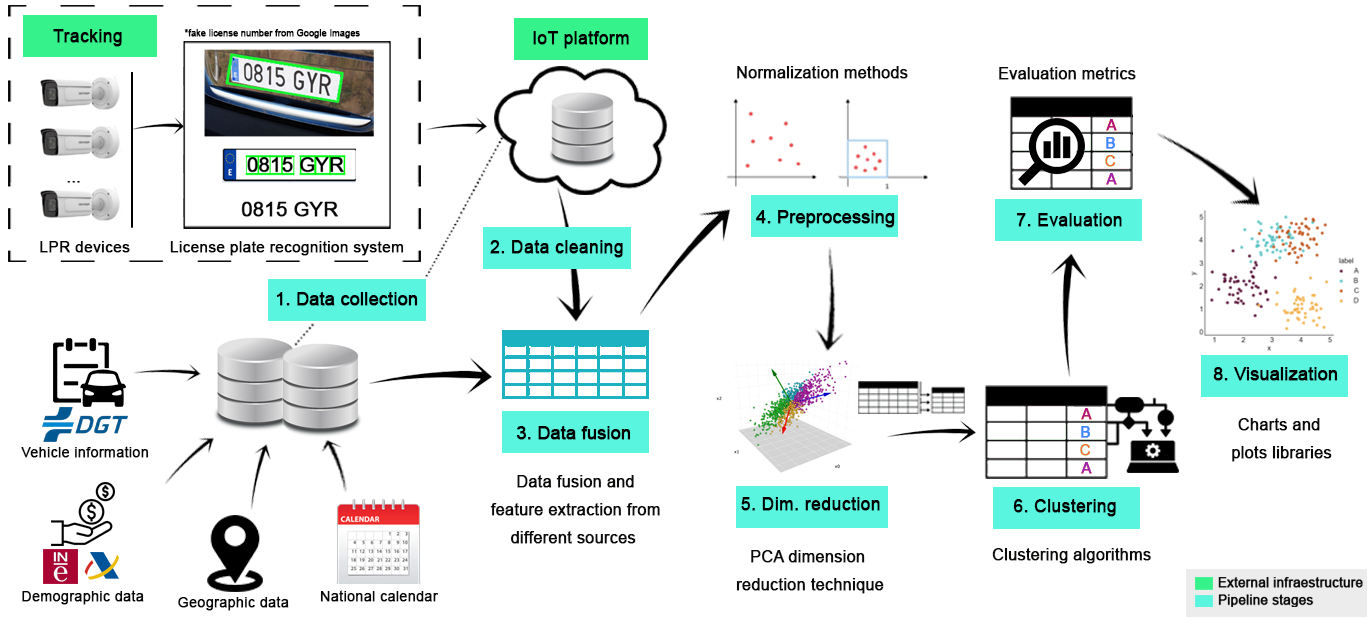
\includegraphics[width = \linewidth]{Images/arquitectura.png}
\end{center}
	\caption{\label{fig:arquitectura} Overview of the clustering pipeline.}
\end{figure}

% Please add the following required packages to your document preamble:
% \usepackage{graphicx}
\begin{table}[]
\centering
\resizebox{\columnwidth}{!}{%
\begin{tabular}{ccc}
\hline
Stage               & Configuration parameters       & Experimental values                                                                                                                                             \\ \hline
Data Collection         & \begin{tabular}[c]{@{}c@{}}Data collection \\ from different sources   \end{tabular}             & \begin{tabular}[c]{@{}c@{}}Storage in own DB and \\ external IoT platform \end{tabular}
                                                \\ \hline
Data Cleaning         & \begin{tabular}[c]{@{}c@{}}Recovery and treatment \\ of lost data   \end{tabular}                & \begin{tabular}[c]{@{}c@{}}1. License plate matching \\ 2. Recover movement of vehicles not \\ detected by any camera in their total route\end{tabular}
\\ \hline
Data Fusion         & \begin{tabular}[c]{@{}c@{}}Fusion of information data \\ and feature extraction   \end{tabular}                & Detailed process in \cref{tab:data-fusion-process}                                                                                                                                                    \\ \hline
Preprocessing       & Normalization methods          &  \begin{tabular}[c]{@{}c@{}}Min-max normalization, z-score standarization, \\ MAD normalization, $\ell^2$ normalizacion        \end{tabular}                                                                                                                                                  \\ \hline
Dimension reduction & \begin{tabular}[c]{@{}c@{}}Dimension reduction \\ techniques \end{tabular} & Principal Component Analysis (PCA)                                                                                                                                                                     \\ \hline
Clustering          & Clustering algorithms          & \begin{tabular}[c]{@{}c@{}}K-Means, MiniBatchKMeans, \\ Agglomerative clustering, BIRCH, \\ DBSCAN, HDBSCAN, MeanShift, \\ Gausian Mixture, Spectral Clustering        \end{tabular}                                                                                                                                                                    \\ \hline
Evaluation          & Evaluation metrics             & \begin{tabular}[c]{@{}c@{}}Silhouette, Davies–Bouldin, \\ Calinski–Harabasz, number of clusters, \\ Bayesian Information Criterion,\\ Akaike Information Criterion\end{tabular} \\ \hline
Visualization       & Visualization plots        & \begin{tabular}[c]{@{}c@{}}box plot, scatter-plot, \\ elbow method, PCA variance plot        \end{tabular}                                                                                                                                                      \\ \hline
\end{tabular}%
}
\caption{Configuration of each stage of the pipeline with the values used in this study.}
\label{tab:pipeline-tab}
\end{table}

\section{Data collection} 
\label{sec:DataCollection}
 The data collection phase handles the collection and storage of our different data sources. This process involves collecting data from different sensors and other data sources, such as Web pages or databases. In our case, we collected the data from LPR cameras and from specific databases we collected: vehicle information, demographic and economic, national calendar, and geographic data.

Regarding vehicle tracking infrastructure (LPR cameras), data is collected by four devices equipped with vehicle detection sensors. These devices are Hikvision LPR IP cameras with Automatic number-plate recognition (ANPR) based on Deep Learning. The devices have a 2MP resolution, 2.8-12 mm varifocal optics, and IR LEDs with a range of 50 m.

To cover the entrances and exits of each village in the target area, we strategically positioned the four cameras, as shown in \cref{fig:map}. The locations are (i) entrance to Pampaneira from the western part of the Alpujarra, (ii) entrance to Pampaneira from the eastern part of the Alpujarra, (iii) entrance to Bubión via a single road, and (iv) entrance to Capileira via a single road. By taking advantage of the road structure, we can monitor the mobility of all vehicles that circulate in the Poqueira area using only four LPRs.

\begin{figure}
\begin{center}
	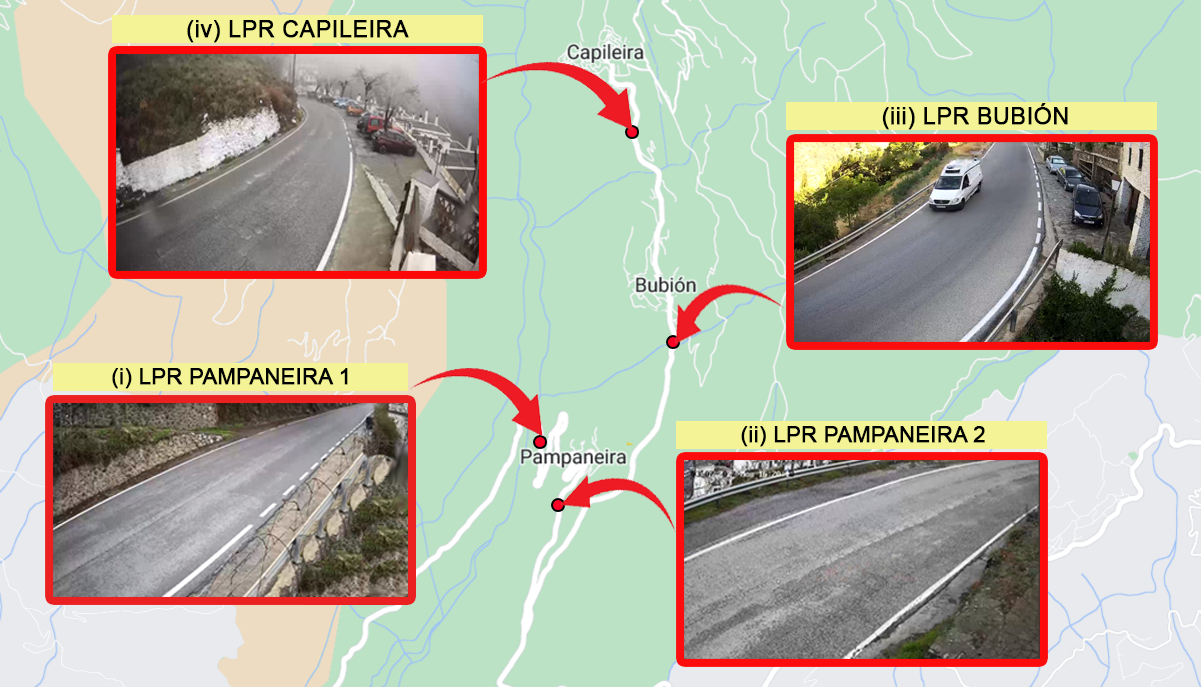
\includegraphics[width = \linewidth]{Images/setup_map.png}
\end{center}
	\caption{\label{fig:map} Setup of the 4 LPR that obtain the data from the license plates of the vehicles.}
\end{figure}

The main objective of these cameras is to track vehicles entering and leaving each of the villages, providing detailed knowledge of mobility in the Poqueira area. Using only four cameras also helped minimize the cost and complexity of the system while still capturing the necessary data. The information collected by the cameras is stored on a cloud platform.

The rest of the data were collected from different databases. Vehicle information from a private dataset of the National Traffic Department. The demographic and economic information from the Internet website of the National Statistics Institute and the Tax Agency. the national calendar and the geographic data are from Python libraries.  


\section{Data Cleaning} 
\label{sec:DataCleaning}
In the field of the IoT, the production of sensor data can often be inaccurate and lead to the loss of some records. In our case, we present two cleaning steps for the main dataset (LPR cameras). The first step, ``license plate matching", aims to reduce the error rate of incomplete or wrongly detected license plates by the LPR devices to maintain consistency between vehicles with the same license plate. About 2\% of the stored 1,050,760 records have missing values in the license plate number. For example, if we have a record with a correct license plate 0000AAA, and another record with the value 0\#00AAA, missing the second digit, we could, by probability, infer that both records belong to the same plate number and assign the correct value, 0000AAA, to both records. In our case, we assign the same plate number to all those records whose license plate matches at least four characters out of seven in the same position. The second step, ``route recovery", aims to reduce the percentage of vehicles not detected by any LPR device. These errors occur when the camera does not detect a vehicle that passes through the road. This error is difficult to detect, but in our setup, if a vehicle moves on the road from camera 1 to 3, and camera 2 (in the middle of the unique road connecting cameras 1 and 3), does not detect the car, we could infer that the car has passed through camera 2. In our process, if the vehicle is detected in less than 30 minutes in two non-consecutive cameras, our system infers that the vehicle is still in the area and calculates its time of stay based on the new registered values.

\section{Data Fusion} \label{sec:DataFusion}

The area where we conducted the experiments, as presented in Section \ref{sec:smartvillages}, records individuals with diverse behavioral patterns and experiences a large flow of tourists from different parts of Spain and elsewhere, each with unique mobility characteristics that vary by region of provenance. Combining data from provenance, mobility in the area, and the holiday calendar offers the opportunity to gain an understanding of the region, its inhabitants, and visitors. This section explains each source of information and the feature extraction and construction process of each dataset to allow the merging. We will detail the structure and variables obtained for each data source, creating a joint database. \cref{tab:data-fusion-process} schematically shows the information fusion process we have followed.


% Please add the following required packages to your document preamble:
% \usepackage{graphicx}
\begin{table}[]
\centering
\resizebox{\columnwidth}{!}{%
\begin{tabular}{lll}
\hline
\multicolumn{1}{c}{Phase} &
  \multicolumn{1}{c}{Tasks} &
  \multicolumn{1}{c}{Values} \\ \hline
\multicolumn{3}{c}{Calendar Data} \\ \hline
Importing Data &
  \begin{tabular}[c]{@{}l@{}}Read the dataset with information on \\ public holidays at national level in Spain\end{tabular} & \begin{tabular}[c]{@{}l@{}}270 days, 3 attributes \\ (date, type, holiday\_period) \end{tabular} \\ \hline
\begin{tabular}[c]{@{}l@{}}Set holiday \\ periods\end{tabular} &
  \begin{tabular}[c]{@{}l@{}}Establish the important holiday \\ periods in Spain: Summer Holiday, \\ Christmas and Holy Week\end{tabular} &
  \begin{tabular}[c]{@{}l@{}}Summer Holiday (from 1 aug. to 31 aug.)  \\ Christmas (from 12 dec. to 6 jan.)\\ Holy Week (from 10 apr. to 17 apr.)\end{tabular} \\ \hline
  \begin{tabular}[c]{@{}l@{}} Encode variables\end{tabular} &
  \begin{tabular}[c]{@{}l@{}}Convert categorical holiday periods \\ into binary variables\end{tabular} & \begin{tabular}[c]{@{}l@{}}270 days, 5 attributes \\ (date, type, Summer, Christmas, Holy\_Week) \end{tabular} \\ \hline
\multicolumn{3}{c}{License Plate Recognition Data} \\ \hline
Importing Data &
  \begin{tabular}[c]{@{}l@{}}Read the cleaned dataset produced \\ from the detection of vehicle license plates \end{tabular} &\begin{tabular}[c]{@{}l@{}}
  1,050,760 rows, 4 attributes \\ (license\_plate, time\_stamp, type, camera\_id)\end{tabular} \\ \hline
\begin{tabular}[c]{@{}l@{}}Calculate \\ associate variables\end{tabular} &
  \begin{tabular}[c]{@{}l@{}}Calculate variables combining the 4 cameras\end{tabular} & \begin{tabular}[c]{@{}l@{}}(license\_plate, entry\_time\_stamp, exit\_time\_stamp, \\ route, total\_distance)\end{tabular}
   \\ \hline
Group information &
  Group the information for each record by vehicle & \begin{tabular}[c]{@{}l@{}}50,901 rows, 10 attributes \\ (license\_plate, total\_entries, avg\_visit\_POQ, \\ std\_visit\_POQ, total\_time\_POQ, nights, route, \\ total\_distance, visits\_dif\_weeks, visits\_dif\_months)\end{tabular}
   \\ \hline
\multicolumn{3}{c}{Vehicle information Data} \\ \hline
Importing Data &
  \begin{tabular}[c]{@{}l@{}}Reads the dataset with vehicle \\ information and its origin\end{tabular} & \begin{tabular}[c]{@{}l@{}}
  45,132 license plates, 4 attributes \\ (license\_plate, postcode, co2\_emissions, num\_seats) \end{tabular} \\ \hline
\multicolumn{3}{c}{Demographic and Economic data} \\ \hline
Importing Data &
  \begin{tabular}[c]{@{}l@{}}Reads demographic information about \\ the region of origin of the vehicle\end{tabular} & \begin{tabular}[c]{@{}l@{}}
  11,752 regions, 4 attributes \\ (postcode, population, gross\_income, disposable\_income)\end{tabular} \\ \hline
  Merging Data &
  \begin{tabular}[c]{@{}l@{}}Merge the two sources \end{tabular} & INE
   \\ \hline
   Validate Data &
  \begin{tabular}[c]{@{}l@{}}Validate information \\ common to the two sources\end{tabular} & INE
   \\ \hline
\multicolumn{3}{c}{Geographic data} \\ \hline
Importing Data &
  \begin{tabular}[c]{@{}l@{}}Reads information regarding the \\ region of origin of the vehicle\end{tabular} &
   \begin{tabular}[c]{@{}l@{}}
  11,752 regions, 8 attributes \\ (postcode, autonomous\_community, province, \\ county, district, town, latitude, longitude)\end{tabular} \\ \hline
    Merging Data &
  \begin{tabular}[c]{@{}l@{}}Mix and validate information \\ from the two sources used\end{tabular} & geopy and pgeocode
   \\ \hline
Standardize values &
  \begin{tabular}[c]{@{}l@{}}Treatment of equivalences between names \\ of regions in different co-official languages\end{tabular} & \begin{tabular}[c]{@{}l@{}}Elimination of accents, spaces and translation \\ to Spanish of all values related to region names\end{tabular}
   \\ \hline
Validate Data &
  \begin{tabular}[c]{@{}l@{}}Validate postcodes and geolocation\end{tabular} & geopy, pgeocode and INE
   \\ \hline
\begin{tabular}[c]{@{}l@{}}Generate \\ new variables\end{tabular} &
  \begin{tabular}[c]{@{}l@{}}Calculate the distance between the study area \\ and the postcode origin from the coordinates\end{tabular} &\begin{tabular}[c]{@{}l@{}}
  11,752 regions, 9 attributes \\ (postcode, autonomous\_community, province, \\ county, district, town, latitude, longitude, km\_to\_POQ)\end{tabular} \\ \hline
\multicolumn{3}{c}{Fusion Dataset} \\ \hline
Merging Data &
\begin{tabular}[c]{@{}l@{}}Unification of header names and data formats, \\Mix postcode and license plate fields, \\Delete rows with some null fields\end{tabular}
   &
  \begin{tabular}[c]{@{}l@{}}
  49,224 vehicles, 24 attributes \\ (license\_plate, total\_entries, avg\_visit\_POQ, std\_visit\_POQ, \\ total\_time\_POQ, nights, route, total\_distance, \\ visits\_dif\_weeks, visits\_dif\_months, co2\_emissions, num\_seats, \\ postcode, autonomous\_community,  province, county, \\ district, town, latitude, longitude, km\_to\_POQ, \\ population, gross\_income, disposable\_income)\end{tabular} \\ \hline 
  \begin{tabular}[c]{@{}l@{}}Generate \\ new variables\end{tabular} &
  \begin{tabular}[c]{@{}l@{}}Calculate variables related to the type \\ of dates in the calendar during the period \\ of stay of each vehicle\end{tabular} & \begin{tabular}[c]{@{}l@{}}
  49,224 vehicles, 29 attributes \\ (license\_plate, total\_entries, avg\_visit\_POQ, std\_visit\_POQ, \\ total\_time\_POQ, nights, route, total\_distance, \\ visits\_dif\_weeks, visits\_dif\_months, co2\_emissions, num\_seats, \\ postcode, autonomous\_community,  province, county, \\ district, town, latitude, longitude, km\_to\_POQ, \\ population, gross\_income, disposable\_income, \\ total\_holiday, total\_workday, entry\_in\_holiday,\\ total\_high\_season, total\_low\_season)\end{tabular}
   \\ \hline
Exporting Data &
  Obtaining the resultant dataset & CLUSTERING\_VEHICLES DB
  \\ \hline
\end{tabular}%
}
\caption{Detailed schematic of the data fusion stage in the pipeline.}
\label{tab:data-fusion-process}
\end{table}


\subsection*{License Plate Recognition Data} \label{subsec:setup}

The LPR cameras described in Section \ref{sec:DataCollection} return information on four variables: the vehicle license plate (license\_plate), the time stamp (time\_stamp), and the direction (type) for each camera defined by an identifier (camera\_id). The dataset contains information for nine months (February to October 2022). On these data, we perform the data cleaning that we defined in Section \ref{sec:DataCleaning}. We change the original license plate value to an integer value that functions as the vehicle identifier. In total, we have 1,050,760 records, of which 25.69\% correspond to the camera PAMPANEIRA 1 (i), 29.25\% to PAMPANEIRA 2 (ii), 19.16\% to BUBION (iii) and 25.9\% to CAPILEIRA (iv) (see in \cref{fig:map}). We grouped the records based on the new vehicle identifier (num\_plate\_ID), taking into account the mobility behavior of each vehicle. For each vehicle, we built a record per each time the vehicle visits the area, containing the date of entry (entry\_time\_stamp) and exit (exit\_time\_stamp) to the area and a list of all the cameras (route) by which it has been registered during its stay, from which we can calculate the distance in kilometers traveled (total distance) in the area. From the above records, we can also calculate the duration of stay (avg\_visit\_POQ) expressed in days and the number of nights spent there. In case of missing data, i.e., we cannot calculate the time of entry or exit of a vehicle in the area, we remove the individual from the dataset.

After that, we performed a grouping at the license plate level so that each database row corresponds to a different individual. In this way, we fuse the information of all the vehicle visits in the area. Finally, we obtained a dataset with the total number of visits (total\_entries), the average time (avg\_visit\_POQ) in days, the complete vehicle routing (route), the total accumulated distance traveled (total\_distance), the standard deviation of the average time of each visit (std\_visit\_POQ) in days, the total time spent (total\_time\_POQ) in the area and the total number of nights spent there (nights). From the new record structure, we can calculate the visits of each vehicle in different weeks (visits\_dif\_weeks) and months (visits\_dif\_months) to study the fidelity of the individual in the area. Finally, we obtain a dataset with 50,901 vehicle records and ten attributes.

\subsection*{Vehicle Information Data} \label{sec:DGT}

The National Department of Traffic in Spain (DGT) has provided us with data relating to vehicle information\footnote{\url{https://sede.dgt.gob.es/es/vehiculos/informe-de-vehiculo/}} including details such as the vehicle's CO2 emissions (co2\_emissions), the number of seats (num\_seats) and the postcode of the vehicle's address (postcode). It is important to note that each vehicle is associated with a fiscal address used to pay road tax.  This will generally match the place of origin of the vehicle driver, although as we have described in Section \ref{sec:smartvillages}, this is not entirely true. This dataset will help us understand the distribution of vehicle types and ownership in the different regions. We have a dataset with 45,132 vehicles registered in Spain and four attributes. Unfortunately, we do not have this information for vehicles registered outside of Spain. The percentage of foreigners in the data sample is less than 9.5\%. Therefore, we determined these individuals exclusively by their mobility behavior in the area. All information related to vehicle information, demographic, economic, and calendar holidays is restricted to Spanish-registered vehicles.   

\subsection*{Demographic and Economic data}

We have access to data regarding population size (population), average gross income (gross\_income), and average disposable income (disposable\_income) per person for each region linked to a postcode (postcode). This information comes from different sources such as the Spanish Tax Agency (AEAT)\footnote{\url{https://sede.agenciatributaria.gob.es/Sede/estadisticas.html}} or the National Statistics Institute (INE)\footnote{\url{https://www.ine.es/dynt3/inebase/es/index.htm?padre=7132\&capsel=5693}}. The data are available for regions with more than 1000 inhabitants and are updated until 2020. When using the AEAT source, we noted that some regions were missing, so we relied solely on the INE as a source for the variables mentioned.  The information collected in this database allows us to understand each region's economic and demographic characteristics, which can be valuable for analyzing patterns in the data related to the drivers' economic capacity and willingness to travel. We obtained a database with 11,752 postcode records from Spain and four attributes. 

\subsection*{National calendar data}

We obtain the holiday data using  a holiday library, which also allows the creation of custom calendars for local holidays, long weekends, and bank holidays. The library is designed to quickly and efficiently generate holiday sets specific to each country and subdivision (such as state or province)\footnote{\url{https://python-holidays.readthedocs.io/en/latest/}}. It aims to determine whether a particular date is a public holiday and to set national and regional holidays for multiple countries. As we mentioned before, due to the small percentage of foreign individuals in the sample, and the complexity of dealing with a different set of holidays for different vehicles, we have restricted the analysis of the holidays to Spain. However, in the holidays, we include Saturdays and Sundays, so we also consider the idea of a weekly holiday for any origin. For each day, represented by a date (date), we have information (type) on whether it is a holiday or a working day in Spain. In addition, holiday periods have been defined to establish high and low tourist seasons based on the three most important national holidays in Spain: Summer, Christmas, and Holy Week\footnote{\url{https://es.statista.com/temas/3585/vacaciones-en-espana/\#topicOverview}}, which represent a binary variable, indicating whether the date belongs to that holiday period (Summer, Christmas, Holy Week). We obtain a database with 270 days and five attributes.

\subsection*{Geographic data}

We get the geographic origin of the vehicles using the postcode and two libraries: pgeocode and geopy. pgeocode\footnote{\url{https://pgeocode.readthedocs.io/en/latest/}} allows fast and efficient queries of GPS coordinates, region name, and municipality name from postcodes. The library can also calculate the distances between postcodes. geopy\footnote{\url{https://geopy.readthedocs.io/en/latest/}} is a Python client that provides access to several popular geocoding web services. It allows developers to find the coordinates of addresses, cities, countries, and landmarks from third-party geocoders and other data sources. The library includes geocoding classes for numerous services, such as OpenStreetMap Nominatim and Google Geocoding API (V3), which can be found at geopy.geocoders. We use data from both sources to validate and complement each other's vehicle location information at different levels, such as municipality, county, or suburb. Furthermore, we also use data from the National Statistics Institute (INE)\footnote{\url{https://www.ine.es/daco/daco42/codmun/cod\_ccaa\_provincia.htm}} to verify the province and autonomous community code of the vehicle, which is directly related to the postcode. Hence, we have created a database that contains, for each postcode, information about: (autonomous\_community), (province), (county), (district), (town), (latitude), (longitude), and distance in kilometers between the origin of the vehicle and the study area (km\_to\_POQ). We obtain a database with 11,752 postal code records for Spain and nine attributes.

\subsection*{Merge of all the processed datasets}

Finally, we fuse all constructed databases, crossing the information from the license plate and postcode variables. After merging the tables, we eliminated records with any of the aforementioned attributes null. The information from the national calendar allows us to add to the vehicle database information related to the stay and its total number of holidays (total\_holiday), workdays (total\_workday), high season (total\_high\_season), low season (total\_high\_season) and a binary variable indicating whether the vehicle enters the area on a holiday or a workday (entry\_in\_holiday). The resulting dataset contains information on the behavior in the area for 49,224 vehicles and 29 attributes. 

\section{Preprocessing} \label{sec:preprocessing}

Our dataset contains about 29 attributes with different scales and units. Hence, some variables may be more influential than others in our analysis. To solve this problem, we will apply normalization to the data. Normalization must be applied to numerical data, so we must first convert the categorical variables to numerical values. Of the 29 variables, only the following are categorical: postcode, route, autonomous\_community, province, county, district, town, license\_plate. The variable license\_plate is a unique identifier of each record, so we delete it. The region variable directly correlates with the km\_to\_POQ, so we can eliminate this feature without losing information. For the same reason, we eliminated the variables latitude and longitude. The numeric variable, total\_distance, keeps the information of the kilometers traveled in the variable route. We will not use in this problem the variables co2\_emissions and num\_seats, since they contain empty values for a high percentage of individuals (approx. 25\%). Also, we believe that for this problem, they do not provide information of relevant interest. We will finally obtain a dataset with 49,224 vehicles and 17 numerical attributes: total\_entries, avg\_visit\_POQ, std\_visit\_POQ, total\_time\_POQ, nights, total\_distance, visits\_dif\_weeks, visits\_dif\_months, km\_to\_POQ, population, gross\_income, disposable\_income, total\_holiday, total\_workday, entry\_in\_holiday, total\_high\_season, total\_low\_season. 

\section{Dimensionality reduction} 

%After preprocessing, we reduce the dimensionality of the dataset. 
It is advisable to reduce the search space of the feature matrix before the clustering for efficiency reasons. This process aims to create a simplified set of dimensions containing much of the variance of the original dataset, as there could be features with very low variance, which would make them of little use for our goal of clustering into different vehicle behaviors. Specifically, we want to minimize the number of components as a function of the variance explained. Hence, after the normalization in Section \ref{sec:preprocessing}, we apply Principal Component Analysis (PCA), as a dimensionality reduction algorithm. The result of this stage is a projection of the original dimensions onto a smaller number of new dimensions, also called PCA components. Then, we will evaluate which normalization offers a higher variability value on a fixed value of PCA components. Visualizing the variance explained by each component can help choose the best normalization. This analysis will be discussed in Chapter \ref{ch:results}.

Removing highly correlated features can cause a loss of information for data with high dimensionality, and the PCA technique reduces the dimension of the dataset \cite{frost2017multicollinearity}. However, we have found that removing variables with very high correlation substantially improves the results and the performance of the clustering models for our data. Furthermore, correlated variables increase the data's variance, making the visual interpretation of the PCA results difficult, as the firsts principal components may not accurately reflect the underlying structure of the data.

\section{Clustering and evaluation}

Our choice of unsupervised machine learning is motivated by the need to categorize unlabeled individuals into distinct groups. Our study explores all the algorithms mentioned in Section \ref{subsec:algorithms} to determine the optimal approach for pattern recognition and evaluate whether they can find a realistic solution.

\section{Visualization} 

Data visualization is essential in our work, as it helps to determine and make decisions about parameter settings, algorithms, and normalization used in our analysis. Likewise, it helps in the explainability of the machine learning results. Regardless of the metrics used, performing a visual evaluation of the results is recommended. Combining the evaluation metrics and visualization charts, we can reach conclusions that facilitate making informed decisions on configuring our model. For example, we use the elbow method to determine the optimal number of clusters for different algorithms. This method consists of plotting a graph based on the number of clusters or components and a given evaluation metric, and visually looking for the inflection point on the defined curve (``elbow"). By selecting the number of components at the bend, we strike a balance between model complexity and accuracy. 

We have visualized the first two PCA components for each normalization with scatter plots to study the data's geometry and the clusters' distribution. These visualizations help to understand the underlying structure of the data. However, there is a limitation in the number of coordinates supported for the scatter plot (maximum 3). Some graphs, such as the Andrews curves, exceed the theoretical limit of the number of components displayed, as they are based on the Fourier series. The problem arises because too many individuals in the dataset overlap, which causes the cluster curves to overlap as well and, thus, provide limited visual information. Therefore, this graph is not helpful for our data. We also use box plots to visualize the distribution of each feature among the individuals in each generated cluster. By comparing these distributions between different clusters, we can identify common patterns that help us understand the individuals that compose each cluster.
\chapter{Results} \label{ch:results}

The first intuitive analysis is a correlation to identifying possible predictors of residency. As we want to model the behavior of the traffic, and we assume that the behavior of the residents should be different from the tourists' behavior, we correlate the residence label against all the other variables. We assign a label of 1 if the vehicle is registered in Pampaneira, Capileira or Bubión (registered resident) and 0 otherwise. Our results reveal several variables that showed non-significant correlations (correlation less than 0.2): avg\_visit\_POQ, std\_visit\_POQ, and population, which have been removed (see in \cref{fig:resident_corr}). \cref{tab:outliers} shows the mean and standard deviation for a selection of uncorrelated variables between two groups: registered residents and non-registered individuals. The variable visit\_POQ, which relates to the time of each visit to the area, has a high standard deviation (std\_visit\_POQ) for registered residents, which could indicate the existence of residents who go out more often and others less often. Furthermore, the mean values (avg\_visit\_POQ) of this variable (visit\_POQ) do not differ much between the two groups. As for the population size variable, there are other villages with a similar size to that of the three villages under study. Hence, the three removed variables are less relevant than the rest in predicting whether a vehicle is a resident of the study area or not.

\begin{figure}
\begin{center}
	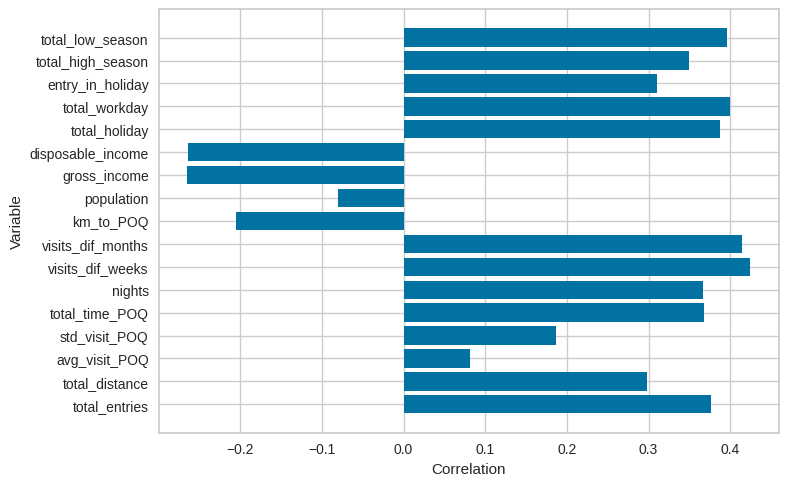
\includegraphics[width = 0.9 \linewidth]{Images/resident_corr.png}
\end{center}
	\caption{\label{fig:resident_corr} Correlation between the registered resident label and the rest of the variables.}
\end{figure}

\begin{table}[]
\centering
\resizebox{\columnwidth}{!}{%
\begin{tabular}{ccccccccc}
\hline
\textbf{}            & \multicolumn{2}{c}{nights}         & \multicolumn{2}{c}{total\_distance} & \multicolumn{2}{c}{total\_entries}     & \multicolumn{2}{c}{entry\_in\_holiday}  \\ \hline
                     & Residents         & Others         & Residents          & Others         & Residents           & Others           & Residents          & Others             \\ \hline
mean                 & 158.47            & 19.99          & 205.82             & 13.60          & 19.46               & 2.35             & 4.26               & 0.72               \\
std                  & 72.37             & 48.07          & 238.52             & 47.78          & 23.57               & 6.58             & 5.49               & 1.70               \\ \hline
\multicolumn{1}{l}{} & \multicolumn{2}{c}{gross\_income}  & \multicolumn{2}{c}{km\_to\_POQ}     & \multicolumn{2}{c}{visits\_dif\_weeks} & \multicolumn{2}{c}{total\_high\_season} \\ \hline
                     & Residents         & Others         & Residents          & Others         & Residents           & Others           & Residents          & Others             \\ \hline
mean                 & 16,084            & 25,007.07      & 1.02               & 374.73         & 4.57                & 1.48             & 27.53              & 3.84               \\
std                  & 0.00              & 7671.19        & 0.59               & 486.97         & 4.03                & 1.97             & 14.75              & 9.00               \\ \hline
\multicolumn{1}{l}{} & \multicolumn{2}{c}{total\_holiday} & \multicolumn{2}{c}{avg\_visit\_POQ} & \multicolumn{2}{c}{std\_visit\_POQ}    & \multicolumn{2}{c}{population}          \\ \hline
                     & Residents         & Others         & Residents          & Others         & Residents           & Others           & Residents          & Others             \\ \hline
mean                 & 52.54             & 6.83           & 23.60              & 10.54          & 20.26               & 4.15             & 406.66             & 19,8175.90         \\
std                  & 23.71             & 15.06          & 34.85              & 31.87          & 23.35               & 16.05            & 121.16             & 56,7183.30    \\ \hline   
\end{tabular}%
}
\caption{Mean and std. deviation for registered residents and rest of individuals in dataset.}
\label{tab:outliers}
\end{table}

\subsection*{Preprocessing and Dimension reduction results: Normalization selection}


Although the preprocessing and dimension reduction stages are performed sequentially, they are interdependent, so we will describe them together. 

PCA technique handles the linear correlations of the original variables to create the principal components. However, we observed that the prior removal of highly correlated variables improves the variance explained by PCA and the scatter plots displaying the PCA component. Hence, we plot in \cref{fig:matrix} the correlation matrix, in which each entry represents the correlation coefficient between a pair of attributes in the dataset. We identify five pairs of variables that are highly correlated, which may cause multicollinearity problems in the study. Specifically, we remove variables that have a correlation coefficient higher than 0.90 with other variables, reducing the attributes in our dataset. We therefore use the following variables: total\_entries, nights, visit\_dif\_weeks, visit\_dif\_months, km\_to\_POQ, gross\_income, entry\_in\_holiday, total\_distance and total\_high\_season.


\begin{figure}
\begin{center}
	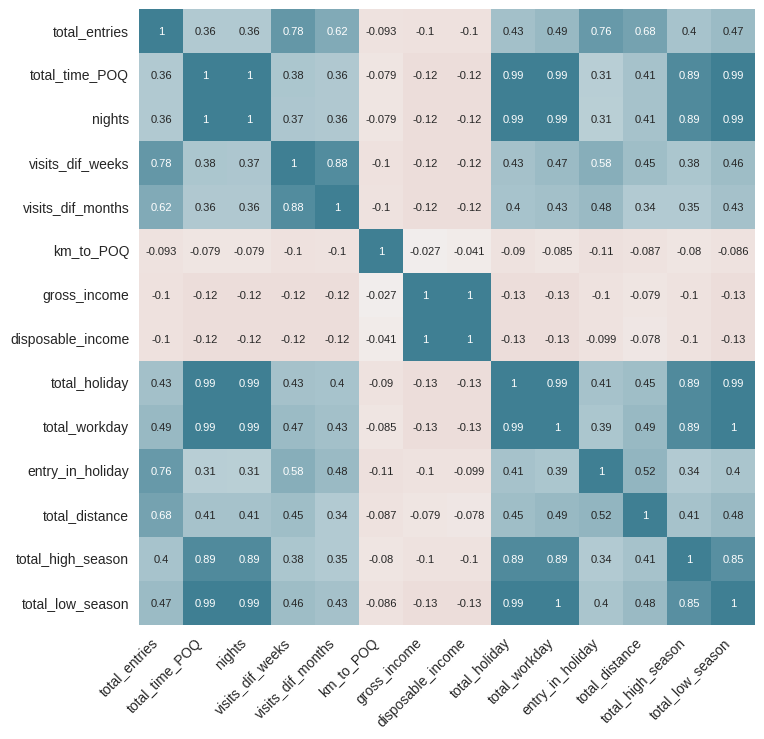
\includegraphics[width = \linewidth]{Images/matriz_corr_v2.png}
\end{center}
	\caption{\label{fig:matrix} Correlation matrix for all variables in the proposed dataset.}
\end{figure}

After applying the four most common normalization to the data (see in Chapter \ref{ch:fundamentals}), we apply PCA analysis. \cref{fig:pca-norms} shows the variance carried by each PCA component for each normalization. We can appreciate that two components explain most of the variance in all normalization. Hence, we perform an exploratory visual analysis plotting the first two principal components to study their underlying geometry. We have overlapped on the plots, in red, the points representing the vehicles of the registered residents. These visualizations provide information about the data structures and the performance of each normalization method. Based on the principal component analysis and the visualization of the data geometry, we will choose which type of algorithm and normalization is the most suitable for our problem (see in \cref{fig:plot-norms}).

\begin{figure}
    \centering
    \subfigure[Min-max normalization.]{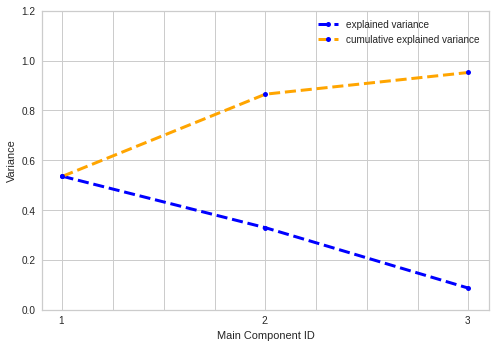
\includegraphics[width=0.49\textwidth]{Images/pca-max.png}}
    \subfigure[Z-score standarization.]{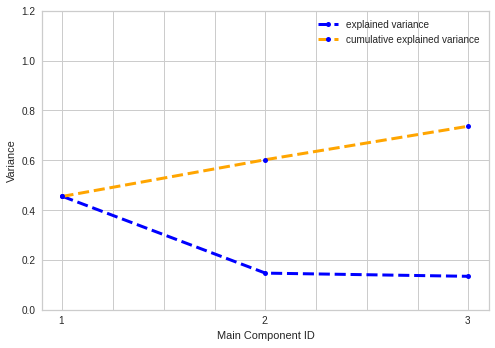
\includegraphics[width=0.49\textwidth]{Images/pca-mean.png}} 
    \subfigure[MAD normalization.]{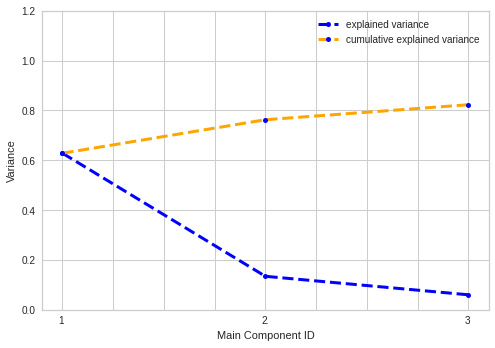
\includegraphics[width=0.49\textwidth]{Images/pca-mad.png}} 
    \subfigure[$\ell^2$ normalization.]{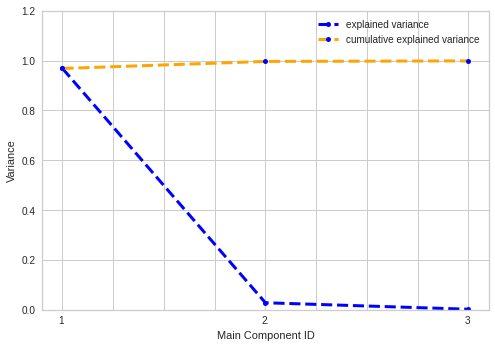
\includegraphics[width=0.49\textwidth]{Images/pca-l2.png}}
    \caption{Variance with 3 principal components.}
    \label{fig:pca-norms}
\end{figure}

\begin{figure}
    \centering
    \subfigure[Min-max normalization.]{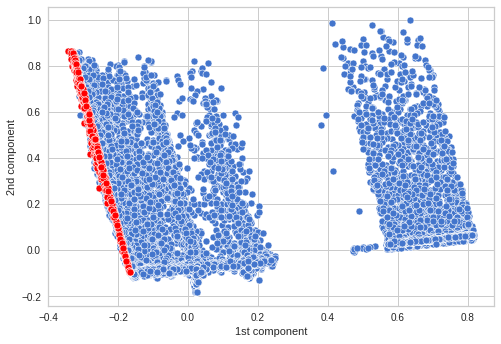
\includegraphics[width=0.49\textwidth]{Images/plot-max.png}}
    \subfigure[Z-score standarization.]{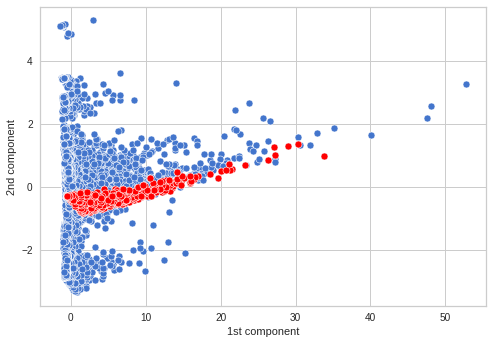
\includegraphics[width=0.49\textwidth]{Images/plot-mean.png}} 
    \subfigure[MAD normalization.]{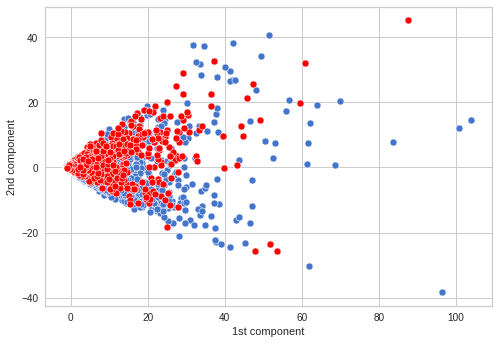
\includegraphics[width=0.49\textwidth]{Images/plot-mad.png}} 
    \subfigure[$\ell^2$ normalization.]{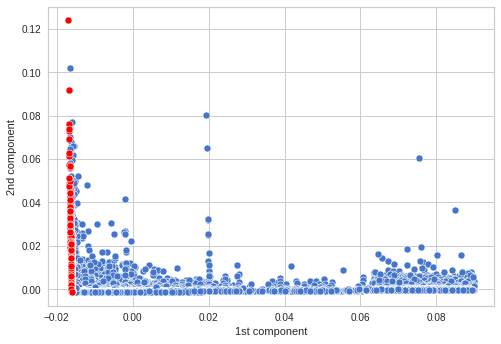
\includegraphics[width=0.49\textwidth]{Images/plot-l2.png}}
    \caption{Scatter-plot of the first two principal components for the different normalizations.}
    \label{fig:plot-norms}
\end{figure}

The normalization method that obtained the highest cumulative variance is $\ell^2$, indicating that it retains the most information in only two components (see in \cref{fig:pca-norms} (d)). In addition, the variance of each dimension is high compared to the other techniques analyzed, suggesting that the data are well distributed in both dimensions. The graph in \cref{fig:plot-norms} (d) shows a clear separation between the two groups, and the registered residents (in red) are well confined. The min-max normalization method obtained the second-best cumulative variance and the highest variance for each dimension, preserving a reasonable amount of information in only two components (see in \cref{fig:pca-norms} (a)). The graph also shows a clear separation between the two groups, and the actual residents are defined along a vertical line on the left cluster in \cref{fig:plot-norms} (a). In contrast, the mad normalization method has a lower cumulative variance and variance for each dimension (see in \cref{fig:pca-norms} (c)) than the $\ell^2$ and min-max normalization methods. The 2-dimensional scatter plot shows no apparent clusters (see in \cref{fig:plot-norms} (c)), and the actual residents are highly dispersed, which makes it unusable for our analysis. We had similar results in a scatter plot of three principal components. Finally, the mean normalization, z-score, method presented the lowest cumulative variance, indicating that it loses more information during dimensionality reduction than other techniques (see in \cref{fig:pca-norms} (b)). The graph shows that the actual residents are grouped together, but for the 2-components, there are no apparent significant clusters (see in \cref{fig:plot-norms} (c)). The trend of the cumulative variance explained is rising, suggesting that the current normalization method could be enhanced by including more components. By adding more dimensions, it may be possible to identify a dimension where the group of registered residents conforms to a clearer distribution. Principal Component Analysis (PCA) typically works better with z-score standardization than with min-max normalization. However, normalization techniques that better handle outliers (such as z-score) may not always be effective for all datasets because it tries to distribute the individuals uniformly, softening the outliers. For example, we observed that the min-max normalization method performed better than the z-score standardization, possibly due to the presence of small clusters that z-score detects as outliers. In particular, the dataset has a low proportion of registered residents (less than 2\% of the total sample), which could be considered outliers (see in \cref{tab:outliers}). In these cases, the min-max normalization method, which is more sensitive to small clusters, may give better results. With all this information, we decided to apply the two best normalizations for our data ($\ell^2$ and min-max) and compare the results obtained in the clustering.

From the scatter plots in \cref{fig:plot-norms}, we observe that the data points are spread relatively flat. This suggests that the data points are concentrated in a lower dimensional space within the original feature space. In other words, the data appears to exist in a more compressed space rather than being spread out across multiple dimensions. Hence, partition and distribution-based clustering models are the most suitable for this geometry (see in Section \ref{sec:flat}). To verify this, we have also tested other algorithms with poor results. For example, density and spectral-based algorithms performed poorly, probably because of the non-flat geometry, but also because they work best for detecting outliers. Hierarchical algorithms performed poorly, probably because of the non-flat geometry, but also they have difficulties with highly concentrated datasets, creating distinct groups only when the separation is very obvious. Consequently, we decided to focus on the partitional and distribution-based algorithms, which work well with flat geometry data. In particular, we try Gaussian mixtures, K-Means, and MiniBatchKMeans.

Gaussian Mixture models are more flexible and can handle different cluster shapes and sizes, while K-Means assumes a spherical shape of the clusters and a uniform size. In addition, Gaussian Mixture models can estimate the probability that a data point belongs to a cluster, which can be useful in specific applications where we need to make decisions based on uncertain data or when we want to assign a data point to multiple clusters with different probabilities. On the tests carried out, we discovered that K-Means and MiniBatchKMeans are not able to find any cluster that contains the majority of individuals of registered residents (see in \cref{fig:plot-norms} (a) and (d)). This is because the distribution of these individuals follows an elliptical geometry, which is not amenable to partition-based algorithms directly. Based on these results, we used the Gaussian Mixture clustering algorithm given the geometry of our data and the distribution followed by registered residents. 

\subsubsection*{Evaluation results}

Once selected the algorithm, we need to select the configuration and hyperparameters of the algorithm. In GaussianMixture algorithm, a ``mixture" refers to a linear combination of several Gaussian distributions, where each component represents a Gaussian distribution in the mixture \cite{Reynolds2009}. Each mixture component is defined by a set of parameters, including its own mean and covariance matrix, which describes how the data are distributed in that space. In practice, the number of mixture components is an adjustable parameter of the algorithm, meaning that we can specify how many Gaussian distributions to combine to model the data. Another configurable parameter of the GaussianMixture algorithm covariance type used to construct the covariance matrix associated with each mixture component. These covariance types specify how the different variables in the data are correlated and can significantly affect the accuracy and efficiency of the model. The common types of covariance are:

\begin{itemize}
    \item Full: all components have their own covariance matrix. This means that each component can have a complex correlation structure between the different variables.
    \item Tied: all components share the same overall covariance matrix. This can be useful if different variables are highly correlated.
    \item Diagonal: each component has its own diagonal in the covariance matrix. This means that the correlation structure between the different variables is limited to correlations between pairs of variables.
    \item Spherical: each mixture component has its own unique variance. This means that the correlation structure between the different variables is limited to the variance of each variable individually.
\end{itemize}

To select the best hyperparameters, we calculate the performance of the resulting model with the metrics presented in Section \ref{subsec:algorithms-mets}, which are appropriated for clustering algorithms based on density (BIC and AIC). In the next subsections, we perform the evaluation for the different types of covariance of the GaussianMixture algorithm on the two normalizations chosen in the previous subsection: min-max and $\ell^2$ normalization.


\subsubsection*{Evaluation results: Min-max normalization}

We begin first by presenting the results obtained with the min-max normalization. \cref{fig:plot-mixmax-bic} represents the values of the BIC and AIC metrics with respect to the number of components and type of covariance used as parameters of the GaussianMixture algorithm. We note that the ``full" covariance type is the one that minimizes both metrics in all cases, so it will be the one chosen for the subsequent analysis. This value means that each component has its own overall covariance matrix, which means it can capture any correlation between variables. We note no significant differences between the values obtained for AIC and BIC scores. Therefore, we calculate the elbow method on the BIC score to select the optimal number of mixture components, which from \cref{fig:plot-mixmax-elbow} is 7, producing an abrupt change in the slope of the curve.

\begin{figure}
    \centering
    \subfigure[BIC score.]{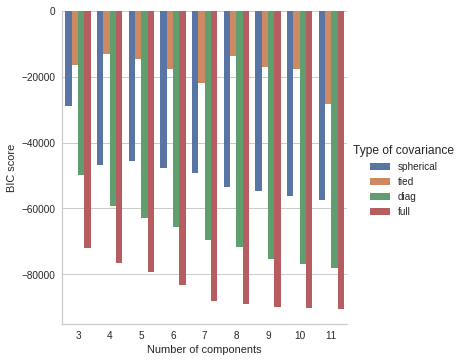
\includegraphics[width=0.49\textwidth]{Images/bic_minmax_2.png}}
    \subfigure[AIC score.]{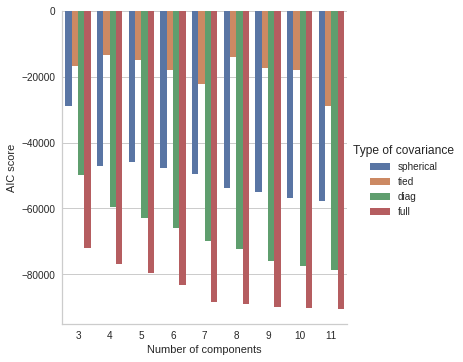
\includegraphics[width=0.49\textwidth]{Images/aic_minmax_2.png}} 
    \caption{Information criteria for the GaussianMixture on min-max normalization.}
    \label{fig:plot-mixmax-bic}
\end{figure}

\begin{figure}
    \centering
    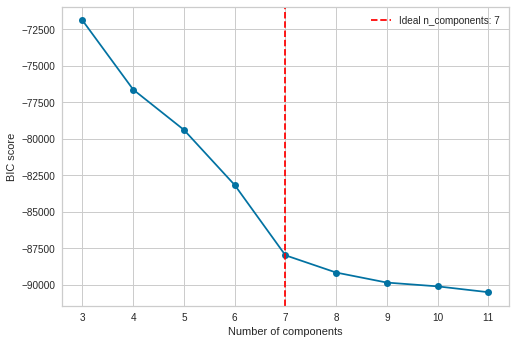
\includegraphics[width=0.6\textwidth]{Images/bic_minmax_elbow_2.png}
    \caption{Elbow method for BIC using min-max normalization.}
    \label{fig:plot-mixmax-elbow}
\end{figure}

\subsubsection*{Evaluation results: $\ell^2$ normalization}

\cref{fig:plot-l2-bic} represents the values of the BIC and AIC metrics with respect to the number of components and type of covariance, used as parameters of the GaussianMixture algorithm for $\ell^2$ normalization. We observe that the ``tied'' covariance type is slightly superior for 3 components, although for more than 3 components the ``full'' covariance type is again the best. Similarly to the min-max normalization, there is no significant difference between the values obtained for AIC and BIC scores. Therefore, we will calculate the elbow method on the BIC score (see in \cref{fig:plot-l2-bic}) and ``full'' covariance type. The elbow method indicates that there is a sharp change in the slope at 4 components.


\begin{figure}
    \centering
    \subfigure[BIC score.]{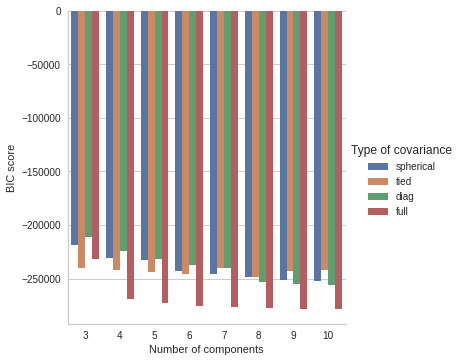
\includegraphics[width=0.49\textwidth]{Images/bic_l2.png}}
    \subfigure[AIC score.]{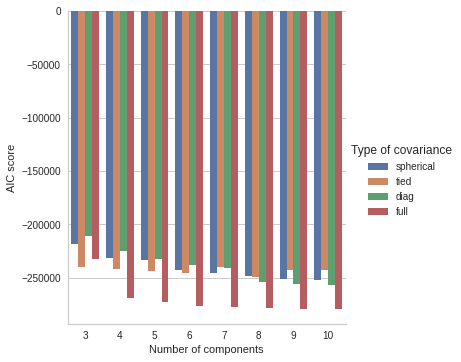
\includegraphics[width=0.49\textwidth]{Images/aic_l2.png}} 
    \caption{Information criteria for the GaussianMixture on $\ell^2$ normalization.}
    \label{fig:plot-l2-bic}
\end{figure}

 

\begin{figure}
    \centering
    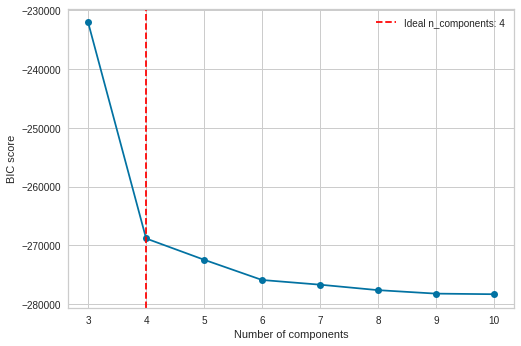
\includegraphics[width=0.6\textwidth]{Images/bic_l2_elbow.png}
    \caption{Elbow method for BIC using $\ell^2$ normalization.}
    \label{fig:plot-l2-elbow}
\end{figure}

\subsubsection*{Visualization results}

Once we have selected the clustering algorithm and the hyperparameters, we will discuss the visualization of the generated clusters over the two chosen normalizations: min-max normalization and $\ell^2$.  

\subsubsection*{Visualization: Min-max normalization}

\cref{fig:plot-scatter-min-max} (a) shows a 2D scatter plot, where each axis represents one of the principal components (1st and 2nd) of the distribution. In \cref{fig:plot-scatter-min-max} (b), we highlight in red the registered residents labeled in our database. Finally, in \cref{fig:plot-scatter-min-max} (c), we can visualize the 3D scatter plot, in which each axis represents one of the 3 principal components. \cref{tab:minmax-perc}, shows the percentage of vehicles and the number of registered residents in each of the 7 clusters. We can see that cluster 3 correctly groups more than 96\% of this group of individuals. Approximately 48\% of the total sample is grouped in only one cluster (cluster 5), so almost half of the vehicles follow the same behavior. In addition, the cluster containing most of the registered residents (cluster 3) represents approximately 11\% of the total population.

\begin{figure}
    \centering
    \subfigure[Segmentation for 7 mixture components.]{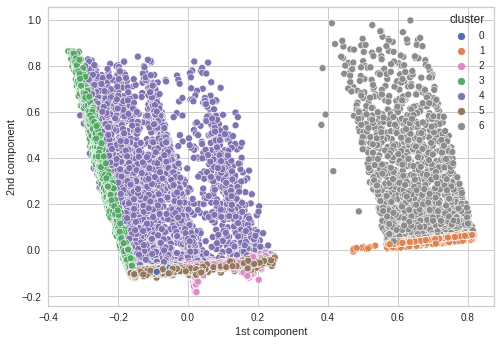
\includegraphics[width=0.49\textwidth]{Images/clustering_sinred_minmax.png}}
    \subfigure[Highlighted registered residents.]{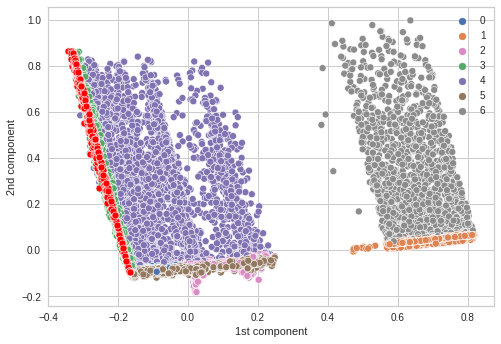
\includegraphics[width=0.49\textwidth]{Images/clustering_red_minmax.png}} 
    \subfigure[3D plot with 3rd component.]{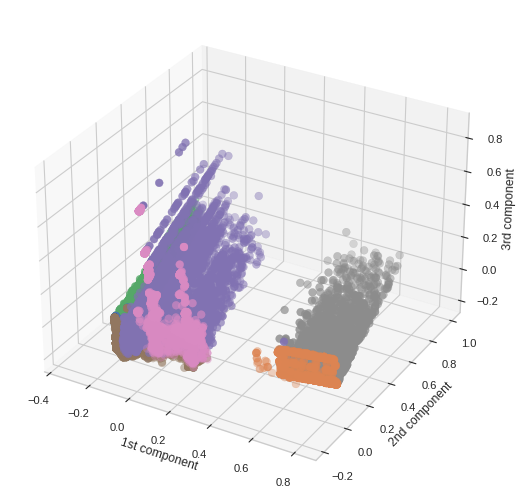
\includegraphics[width=0.49\textwidth]{Images/visual_3D_minmax.png}} 
    \caption{Scatter-plot of the first three components (PCA) using min-max normalization.}
    \label{fig:plot-scatter-min-max}
\end{figure}

% Please add the following required packages to your document preamble:
% \usepackage{graphicx}
\begin{table}[]
\centering
\resizebox{\columnwidth}{!}{%
\begin{tabular}{cccccccc}
\hline
Data points          & \multicolumn{7}{c}{Nº cluster}                                  \\ \hline
                     & 0       & 1      & 2      & 3       & 4      & 5       & 6      \\ \hline
Percentage of sample & 15.04\% & 6.11\% & 8.58\% & 11.17\% & 8.55\% & 47.50\% & 3.05\% \\ \hline
Real Residents       & 10      & 0      & 0      & 641     & 3      & 12      & 0      \\ \hline
Rest of individuals  & 7391    & 3009   & 4221   & 4862    & 4205   & 23,370  & 1500   \\ \hline
\end{tabular}%
}
\caption{Clusters based on registered resident labels using min-max normalization.}
\label{tab:minmax-perc}
\end{table}

\cref{fig:boxplot-minmax} presents the box plots for the 7 clusters for the nights (\cref{fig:boxplot-minmax} (a)) and km\_to\_POQ (\cref{fig:boxplot-minmax} (b)) variables, which show significant differences in explaining the groups. \cref{fig:boxplot-minmax-1,fig:boxplot-minmax-2} present the box plots of the most relevant variables for the 7 clusters obtained, making a previous division into 2 groups, which we explain below. \cref{tab:means-minmax} complements \cref{fig:boxplot-minmax-1,fig:boxplot-minmax-2}, indicating the exact number of the mean of each variable in each cluster. To facilitate visualization, we have separated some of the box plots according to the value of the variable nights, which seems to discriminate well between 2 groups of clusters: (0, 1, 2, 5) with lower values and (3, 4, 6) with higher values (see in \cref{fig:boxplot-minmax} (a)). Clusters 3,4,6 have a number of nights close to the behavior of a resident in the area. These represent 22.77\% of the total sample (see in \cref{tab:minmax-perc}). Clusters 0,1,2,5 have visitor behavior because they spent fewer nights in the area and represent 77.23\% of the total dataset. Thus, we can define a distinction between the 7 clusters based on length of stay, which is directly correlated with overnights.

\begin{figure}
    \centering
    \subfigure[Total nights of stay by cluster.]{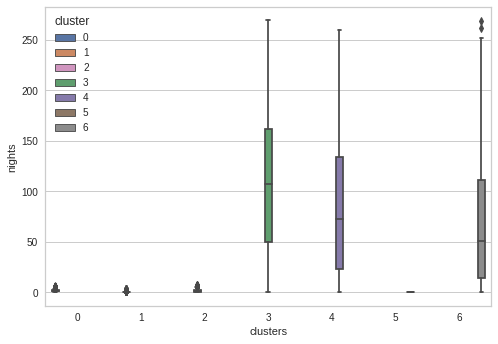
\includegraphics[width=0.49\textwidth]{Images/boxplot_minmax_1.png}}
    \subfigure[Distance in Km. to the area by cluster.]{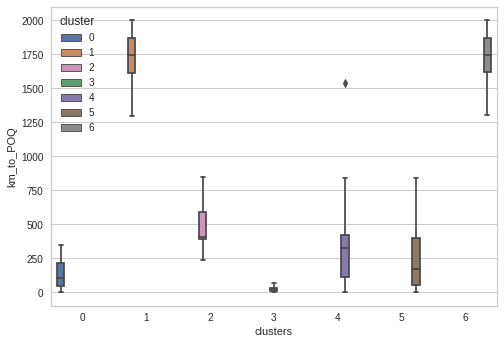
\includegraphics[width=0.49\textwidth]{Images/boxplot_minmax_2.png}}
    \caption{box plots for min-max normalization (I).}
    \label{fig:boxplot-minmax}
\end{figure}


\begin{figure}
    \centering
    \subfigure[Nights of stay for clusters \textbf{3,4,6}.]{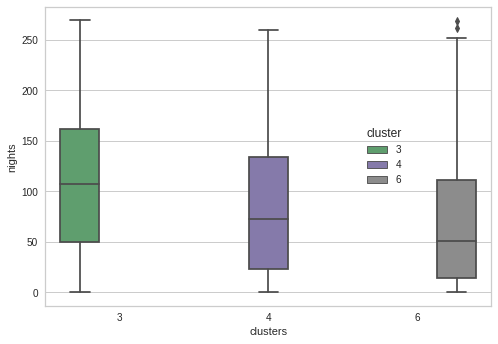
\includegraphics[width=0.49\textwidth]{Images/boxplot_max_1.png}}
    \subfigure[Nights of stay for clusters \textbf{0,1,2,5}.]{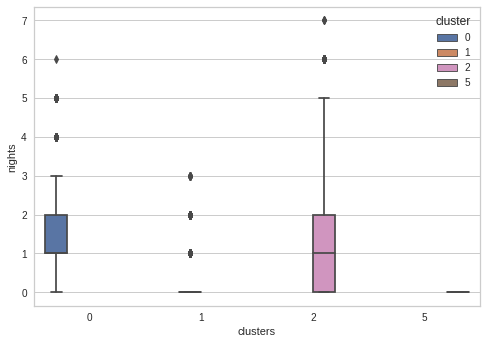
\includegraphics[width=0.49\textwidth]{Images/boxplot_min_1.png}}
    \subfigure[Distance to the area for clusters \textbf{3,4,6}.]{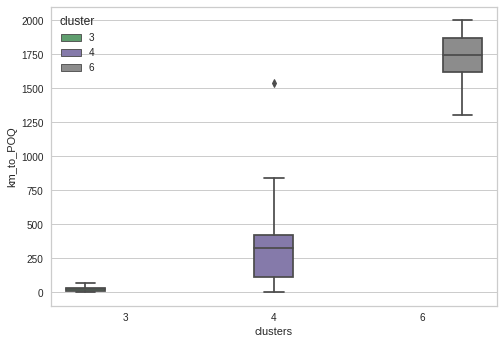
\includegraphics[width=0.49\textwidth]{Images/boxplot_max_2.png}}
    \subfigure[Distance to the area for clusters \textbf{0,1,2,5}.]{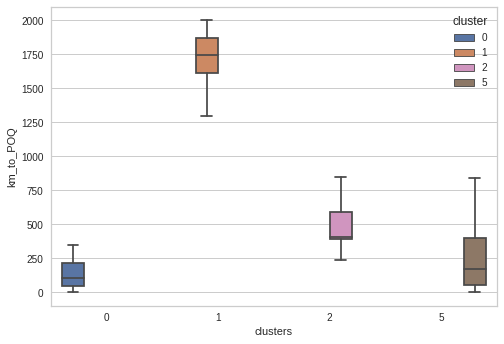
\includegraphics[width=0.49\textwidth]{Images/boxplot_min_2.png}}
    \subfigure[Total entries for clusters \textbf{3,4,6}.]{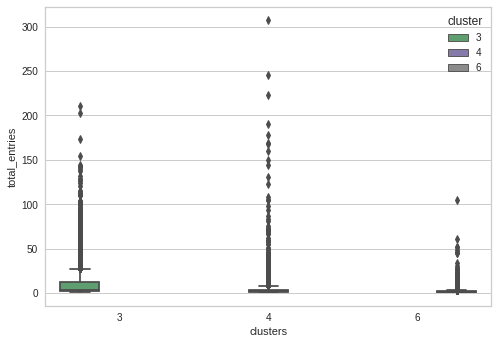
\includegraphics[width=0.49\textwidth]{Images/boxplot_max_3.png}} 
    \subfigure[Total entries for clusters \textbf{0,1,2,5}.]{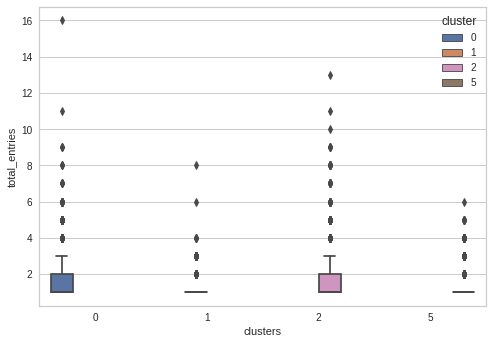
\includegraphics[width=0.49\textwidth]{Images/boxplot_min_3.png}} 
    \caption{Box plots for min-max normalization (II).}
    \label{fig:boxplot-minmax-1}
\end{figure}

\begin{figure}
    \centering
    \subfigure[Distance run in area for clusters \textbf{3,4,6}.]{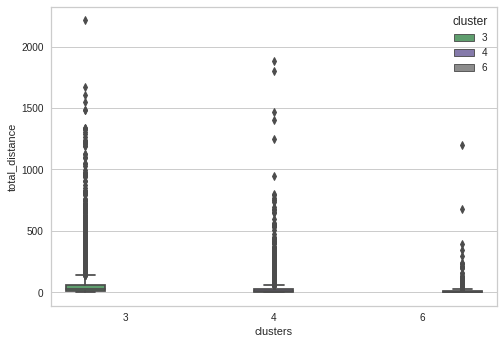
\includegraphics[width=0.49\textwidth]{Images/boxplot_max_4.png}}
    \subfigure[Distance run in area for clusters \textbf{0,1,2,5}.]{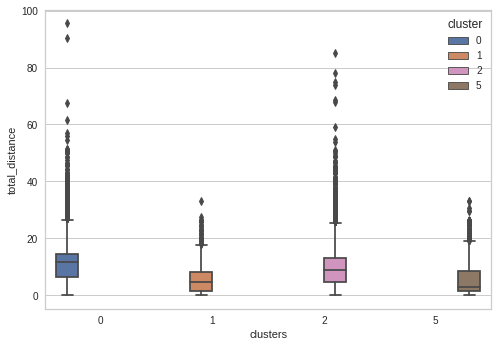
\includegraphics[width=0.49\textwidth]{Images/boxplot_min_4.png}}
    \subfigure[Avg. gross income for clusters \textbf{3,4,6}.]{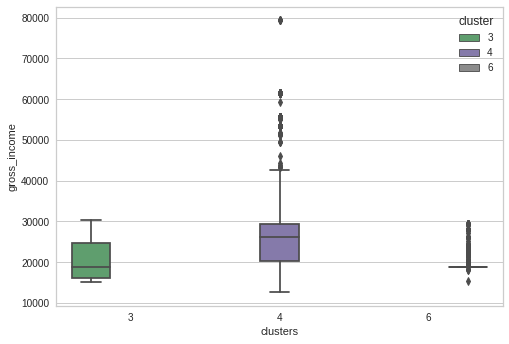
\includegraphics[width=0.49\textwidth]{Images/boxplot_max_5.png}} 
    \subfigure[Avg. gross income for clusters \textbf{0,1,2,5}.]{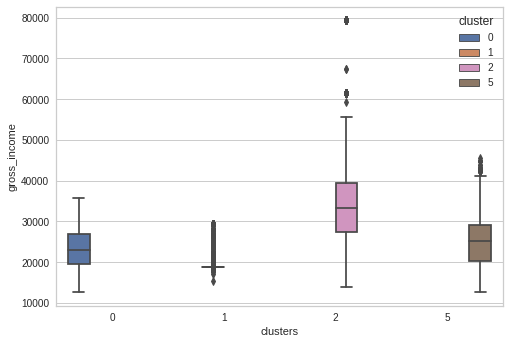
\includegraphics[width=0.49\textwidth]{Images/boxplot_min_5.png}} 
    \subfigure[Total high season for clusters \textbf{3,4,6}.]{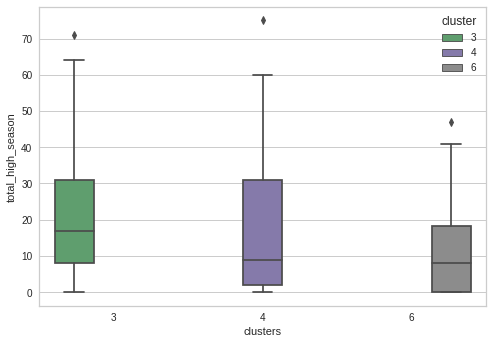
\includegraphics[width=0.49\textwidth]{Images/boxplot_max_6.png}} 
    \subfigure[Total high season for clusters \textbf{0,1,2,5}.]{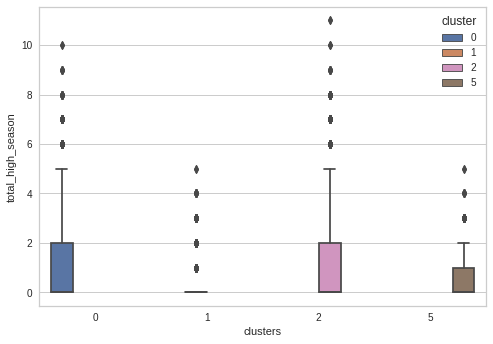
\includegraphics[width=0.49\textwidth]{Images/boxplot_min_6.png}} 
    \caption{Box plots for min-max normalization (III).}
    \label{fig:boxplot-minmax-2}
\end{figure}

For clusters 3,4,6 (residents' behavior), another relevant variable is the distance in kilometers from the registered address of the vehicle to the area (see in \cref{fig:boxplot-minmax-1} (c)). The three clusters, despite having notable differences for the variable of origin, have similar behaviors for the variable of nights. Hence, the individuals in these 3 clusters have residence or accommodation in the area. According to their distance to the area, cluster 3, with a mean value of 19.39 km (see in \cref{tab:means-minmax}), corresponds mostly to vehicles registered in the area under study (registered residents) and nearby villages in the Alpujarra. Cluster 6, with a mean value of 1747.30 km for the variable km\_to\_POQ, corresponds to non-registered residents from abroad that we defined in Section \ref{sec:smartvillages}. Cluster 4, with a mean value of 318.36 km, corresponds to individuals from other regions of Spain who are non-registered residents, which we also discussed in that Section. Moreover, the gross income variable is much higher in group 4 than in groups 3 and 6 (almost 34\% higher) (see in \cref{fig:boxplot-minmax-2} (c)). Therefore, we can say that the majority of individuals in this group (non-registered residents from other Spanish regions) come from regions with higher incomes than the average of the rest of the residents. We can observe that in general for the three groups of residents, the mean of the variables total\_distance, total\_high\_season, and total\_entries (see in \cref{tab:means-minmax}), are inversely proportional to the mean of the clusters for the variable km\_to\_POQ. Therefore, residents coming from farther away (clusters 4 and 6) will have a lower mean than the clusters coming from closer (cluster 3) for those variables, this is because coming from farther away the frequency of visitation, kilometers traveled and visits in high season (see in \cref{fig:boxplot-minmax-1} (e) and \cref{fig:boxplot-minmax-2} (a, e)) will also be lower.

For clusters 0,1,2,5 (visitor behavior), we also describe the average behavior of each cluster (see in \cref{tab:means-minmax}). Cluster 0 has an average distance of 128.55 km to the area, so it corresponds to visitors from the province of Granada (region of the villages). This cluster comprises individuals who spend an average of 1.57 nights in the area. The variable total\_entries tells us that individuals have made an average of 1.54 visits during the period collected in the sample. Due to its variables total\_high\_season (see in \cref{fig:boxplot-minmax-2} (b, f)), we observe that more than 65\% of the visits are made in high season. Therefore, this cluster corresponds to individuals from the province of Granada who visit the area on weekends and holidays and stay between 1–2 nights. Cluster 1 has an average of 1742.97 km, which indicates foreign visitors. This cluster has an average of 0.26 nights, so they are individuals who usually visit the area during the day. Observing the variable total\_high\_season, we can see that the behavior of these individuals who come from abroad is to visit in low seasons. In addition, the relatively low value of the total\_distance variable (4.90 km) suggests that it is likely that these tourists visit one of the three villages, specifically Pampaneira, using the main road instead of deviating from other routes, probably the behavior of these individuals is to visit the towns of the Alpujarra that coincide with the route of the main road. Cluster 2 has an average of 474.21 km, so visitors come from outside the province of Granada. This cluster comprises individuals who spend an average of 1.55 nights in the area, similar to cluster 0 (visitors from the province of Granada). This cluster has the highest average for the gross\_income variable of all the clusters (see in \cref{fig:boxplot-minmax-2} (d)). This leads us to think that it contains vehicles from the north of Spain, where the average income is higher than in the south of Spain. In addition, the variable total\_high\_season, shows that approximately 74\% of the stays are in high season, so these individuals correspond to tourists from the northern regions of Spain who decide to spend 1–2 days in the Alpujarra during their holidays. Finally, cluster 5 has an average of 253.70 km, indicating visitors from other Andalusia provinces. This cluster has an average of 0 nights, so the visits usually occur during the day, with no associated overnight stays. It is important to highlight that cluster 5 represents 47.50\% of the individuals in the sample (see in \cref{tab:minmax-perc}), so we can say that the majority behavior among individuals is not to spend the night in the area. Furthermore, they rarely come in high season (27\% of the total entries) (see in \cref{fig:boxplot-minmax-2} (f)), so the majority will correspond to tourists from other provinces of Andalusia who visit the area and return home at the end of the day.

\begin{table}[]
\centering
\resizebox{\columnwidth}{!}{%
\begin{tabular}{cccccccc}
\hline
Variables           & \multicolumn{7}{c}{Nº cluster}                                                    \\ \hline
                    & 0         & 1         & 2         & 3         & 4         & 5         & 6         \\ \hline
nights              & 1.57      & 0.26      & 1.55      & 108.62    & 84.66     & 0.00      & 68.73     \\ \hline
km\_to\_POQ         & 128.55    & 1742.97   & 474.21    & 19.39     & 318.36    & 253.70    & 1747.30   \\ \hline
total\_entries      & 1.54      & 1.12      & 1.58      & 10.34     & 4.36      & 1.12      & 2.71      \\ \hline
total\_distance     & 11.64     & 4.90      & 10.67     & 70.24     & 30.77     & 4.86      & 14.42     \\ \hline
gross\_income       & 23,085.36 & 19,482.10 & 35,547.66 & 20,972.17 & 26,902.26 & 25,151.75 & 19,179.54 \\ \hline
total\_high\_season & 1.01      & 0.31      & 1.14      & 18.85     & 15.10     & 0.31      & 11.24     \\ \hline
\end{tabular}%
}
\caption{Mean of variables for each cluster performed using min-max normalization.}
\label{tab:means-minmax}
\end{table}

\subsubsection*{Visualization: $\ell^2$ normalization}

\cref{fig:plot-scatter-l2} shows the distribution of the data using the $\ell^2$ normalization. \cref{fig:plot-scatter-l2} (a) shows a 2D scatter plot, where each axis represents one of the principal components (1st and 2nd) of the distribution of the groups. In \cref{fig:plot-scatter-l2} (b), we highlight in red the registered residents. Finally, in \cref{fig:plot-scatter-l2} (c), we can visualize the 3D scatter plot. \cref{tab:l2-perc} shows the percentage of the total sample and the number of registered residents in each cluster. We can see cluster 0 correctly groups more than 88\% of the registered residents. Approximately 80\% of the total sample is grouped in a single cluster (cluster 3). In addition, the cluster containing registered residents (cluster 0) represents approximately 9\% of the total population.

\begin{figure}
    \centering
    \subfigure[Segmentation for 4 mixture components.]{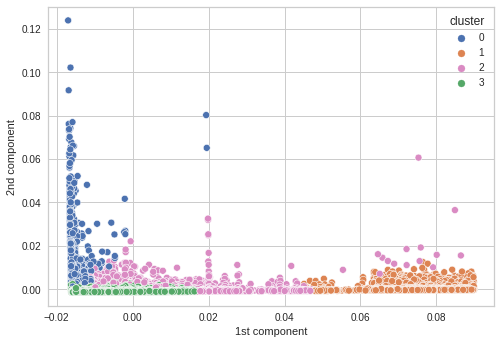
\includegraphics[width=0.49\textwidth]{Images/clustering_sinred_l2.png}}
    \subfigure[Highlighted registered residents.]{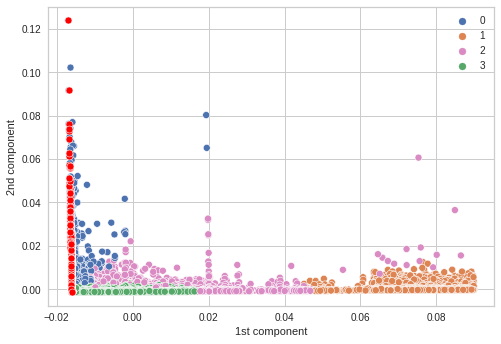
\includegraphics[width=0.49\textwidth]{Images/clustering_red_l2.png}} 
    \subfigure[3D plot with 3rd component.]{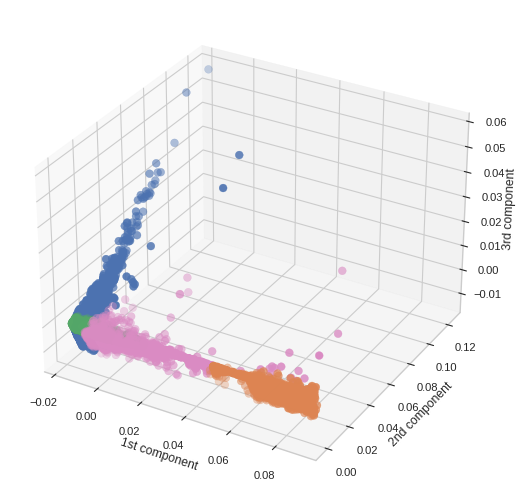
\includegraphics[width=0.49\textwidth]{Images/visual_3D_l2.png}} 
    \caption{Scatter-plot of the first three components (PCA) using $\ell^2$ normalization.}
    \label{fig:plot-scatter-l2}
\end{figure}


\begin{table}[]
%\centering
\resizebox{9cm}{!} & \multicolumn{1}{l}{8.76\%} & \multicolumn{1}{l}{4.36\%} & \multicolumn{1}{l}{78.33\%} \\ \hline
Real Residents                           & 589                        & 0                          & 0                          & 77                          \\ \hline
Rest of individuals                      & 3620                       & 4314                       & 2146                       & 38,478                      \\ \hline
\end{tabular}%
}
\caption{Clusters based on actual resident labels using $\ell^2$ normalization.}
\label{tab:l2-perc}
\end{table}

\cref{fig:boxplot-l2} shows the box plots of the relevant variables for the 4 clusters, and \cref{tab:means-l2} shows the mean of each of these variables in each cluster. We distinguish two clusters that contain a high value of the variable nights (cluster 0 and 2), while the rest of the clusters (clusters 1 and 3) have a low value. Although there are outliers (see in \cref{fig:boxplot-l2} (a)) that increase the mean number of nights for these clusters (clusters 1 and 3), 50\% of the individuals have a number of nights lower than 2 for cluster 3 and lower than 15 nights for cluster 1. 

Cluster 0 has an average of 144.93 nights and an average distance to the area of 25.54 km. In addition, it contains more than 88\% of the real residents. hence, we can consider this cluster as that of the area's residents (registered and unregistered). Most of the unregistered residents in this group, as shown in \cref{fig:boxplot-l2} (b), come from the province of Granada. Cluster 2 is small (only 4.36\% of the total sample) of non-registered residents who spend an average of 84.62 nights and come from an average origin of 598.01 km. Therefore, it corresponds to residents from outside the province of Granada. We can observe that in general, for the two groups, the means of the variables total\_distance, total\_high\_season and total\_entries (see in \cref{tab:means-l2}), are inversely proportional to the means of the variable km\_to\_POQ. This means that visitors that come from further away tend to: visit in the low season; move less inside the area; and come fewer times in the year than other visitors (see in \cref{fig:boxplot-l2} (c, d, f)). Cluster 1 comprises individuals from afar to the 1750.68 km area and has an average of 22.81 nights (although most of them spend less than two nights). This group contains foreign visitors and some unregistered foreign residents (less than half of the group). Only 17\% of the stays are in high season. This is because the cluster comprises foreigners, so they do not depend on the Spanish national calendar. Furthermore, despite having an average of 22.81 nights, the visits to the area are only 1.52, which means that in all those days they do not travel to nearby areas (see in \cref{tab:means-l2}). Finally, group 3 contains the majority of individuals in the data set and models individuals with a mean behavior of 4.82 nights (although most do not stay overnight) and 240.01 km of distance. This cluster represents 78.33\% of the individuals in the sample (see in \cref{tab:l2-perc}). Hence, we can say that the majority behavior of the individuals is not to spend the night in the area. In addition, they rarely come in high season (28\% of the total stay) (see in \cref{fig:boxplot-l2} (f)). Thus, the majority will correspond to tourists from Granada and other nearby Andalusian provinces visiting the area and returning home at the end of the day. Cluster 3 has the highest income, with a mean of 26,158.32; however, since it contains almost 80\% of the sample, it does not provide much information.

\begin{figure}
    \centering
    \subfigure[Total nights of stay by cluster.]{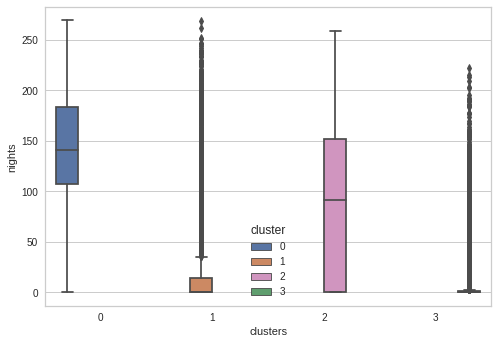
\includegraphics[width=0.49\textwidth]{Images/boxplot_l2_1.png}}
    \subfigure[Distance in Km. to the area by cluster.]{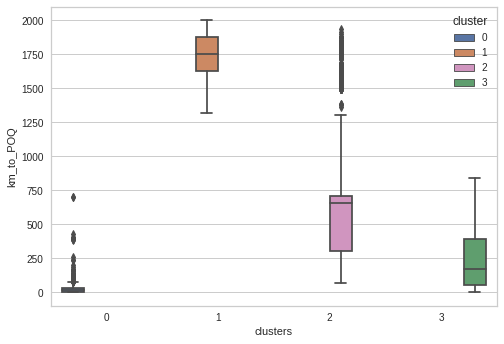
\includegraphics[width=0.49\textwidth]{Images/boxplot_l2_2.png}} 
    \subfigure[Total entries to the area by cluster.]{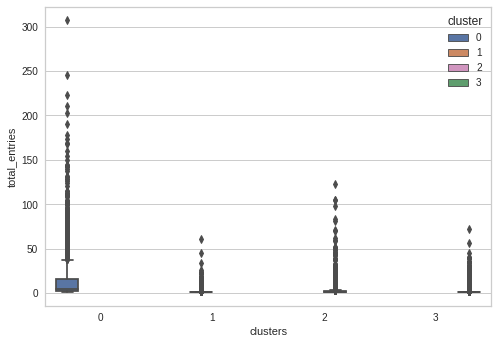
\includegraphics[width=0.49\textwidth]{Images/boxplot_l2_3.png}}
    \subfigure[Distance run in area by cluster.]{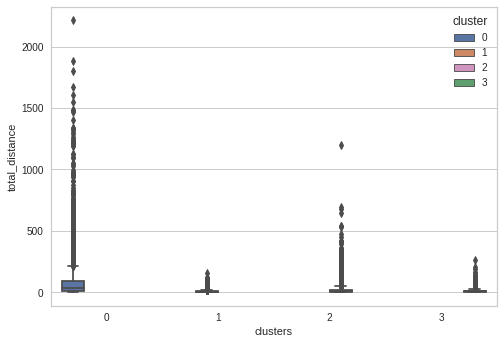
\includegraphics[width=0.49\textwidth]{Images/boxplot_l2_4.png}} 
    \subfigure[Average gross income by cluster.]{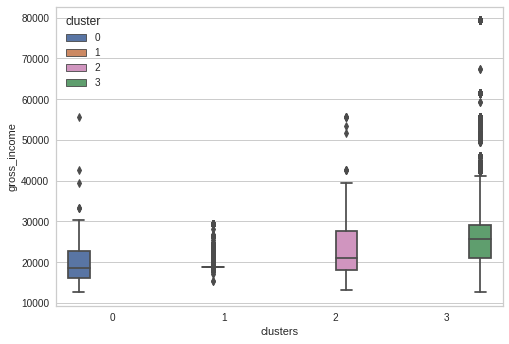
\includegraphics[width=0.49\textwidth]{Images/boxplot_l2_5.png}} 
    \subfigure[Total high season by cluster.]{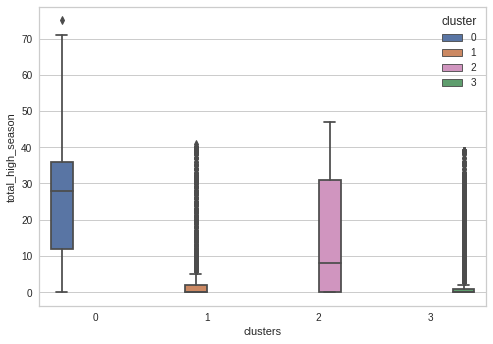
\includegraphics[width=0.49\textwidth]{Images/boxplot_l2_6.png}} 
    \caption{Box plots for $\ell^2$ normalization.}
    \label{fig:boxplot-l2}
\end{figure}

\begin{table}[]
%\centering
\resizebox{10cm}{!}{%
\begin{tabular}{ccccc}
\hline
Variables           & \multicolumn{4}{c}{Nº cluster}                \\ \hline
                    & 0         & 1         & 2         & 3         \\ \hline
nights              & 144.93    & 22.81     & 84.62     & 4.82      \\ \hline
km\_to\_POQ         & 25.54     & 1750.68   & 598.01    & 240.01    \\ \hline
total\_entries      & 13.18     & 1.52      & 3.53      & 1.49      \\ \hline
total\_distance     & 95.43     & 6.89      & 26.43     & 8.01      \\ \hline
gross\_income       & 20,268.41 & 19,018.55 & 22,886.88 & 26,158.32 \\ \hline
total\_high\_season & 24.83     & 3.87      & 14.47     & 1.36      \\ \hline
\end{tabular}%
}
\caption{Mean of variables for each cluster performed using $\ell^2$ normalization.}
\label{tab:means-l2}
\end{table}
\chapter{Discussions}
\label{ch:discussions}

\cref{tab:matching-clusters} shows the equivalence by clusters and percentage of the total set for the two normalizations analyzed. For the group of registered residents, we can see that both normalization methods group them into a single cluster (cluster 3 in min-max and 0 in $\ell^2$). However, there is a 2.62\% difference in the size of these clusters, with the $\ell^2$ cluster size being smaller. The min-max normalization distinguishes between foreign visitors and foreign non-registered residents (clusters 1 and 6, respectively), while the $\ell^2$ normalization groups all foreign individuals into a single cluster (cluster 1). The clusters of national non-registered residents are also similar in both normalization methods (cluster 4 in min-max and 2 in $\ell^2$). Still, there is a 4.19\% difference in the size of these clusters, with the size of the $\ell^2$ cluster also being smaller. Finally, the $\ell^2$ normalization groups all national visitors into a single cluster (cluster 3), while the min-max normalization divides these into three distinct clusters (clusters 0, 2 and 5). It should be noted that in the $\ell^2$ normalization, cluster 3 is larger than the sum of clusters 0, 2 and 5, because it contains individuals with resident behaviors that were not included in the other clusters. This explains the significant differences in the sample sizes of clusters 0 and 2 compared to their equivalents in the min-max normalization.

\begin{table}[]
\centering
\resizebox{\columnwidth}{!}{%
\begin{tabular}{ccccccccc}
\hline
Normalization             &                                 & \multicolumn{7}{c}{}                                                                                                            \\ \hline
\multirow{2}{*}{Min-max}  & \multicolumn{1}{c|}{Nº cluster} & \multicolumn{1}{c|}{3}       & 1      & \multicolumn{1}{c|}{6}      & \multicolumn{1}{c|}{4}      & 0        & 2      & 5       \\ \cline{3-9} 
                          & \multicolumn{1}{c|}{\% sample}  & \multicolumn{1}{c|}{11.17\%} & 6.11\% & \multicolumn{1}{c|}{3.05\%} & \multicolumn{1}{c|}{8.55\%} & 15.04\%  & 8.58\% & 47.50\% \\ \hline
\multirow{2}{*}{$\ell^2$} & \multicolumn{1}{c|}{Nº cluster} & \multicolumn{1}{c|}{0}       & \multicolumn{2}{c|}{1}               & \multicolumn{1}{c|}{2}      & \multicolumn{3}{c}{3}       \\ \cline{3-9} 
                          & \multicolumn{1}{c|}{\% sample}  & \multicolumn{1}{c|}{8.55\%}  & \multicolumn{2}{c|}{8.76\%}          & \multicolumn{1}{c|}{4.36\%} & \multicolumn{3}{c}{78.33\%} \\ \hline
\end{tabular}%
}
\caption{Equivalence of the clusters made for each normalization.}
\label{tab:matching-clusters}
\end{table}

The min-max normalization seems more efficient since it allows a more detailed segmentation of individuals than $\ell^2$, and $\ell^2$ shows more outliers in the box plots for all the variables. While min-max seems to distinguish the residents from the visitors, with the variable representing the number of nights spent in the area, $\ell^2$ seems to have a clear segmentation on the distance to their home. Hence, for our purposes, min-max offers better segmentations. In addition, min-max detects atypical behaviors of individuals not officially registered as residents of the area, but that behave as residents. In contrast, the $\ell^2$ normalization could be useful for excluding foreigners from the analysis and focusing only on comparing registered and non-registered residents at the national level, grouping visitors in a single cluster.

%Añadir sección

% Añadir discussions a resultados y dejar conclusions como que se han ido cumpliendo los objetivos de la introducción. Infraestructura montada y diseñada. Resultados útiles para tal... 
\clearpage

In summary, the work presents an effective pipeline for clustering analysis, using data from different sensors and sources to detect registered and non-registered residents, and visitors; and their behavior in a given area. We have selected an optimal clustering algorithm based on the data distribution and two potential normalization algorithms. We found that the min-max normalization was the most effective for detailed segmentation of individuals and their visiting behavior in the area, and detection of atypical behavior of individuals not registered as residents of the area, but showing resident behavior. The $\ell^2$ normalization could be useful in specific situations requiring a distinction from the region of origin. The information obtained from this analysis can help area managers to create personalized strategies for retaining specific tourists based on income or provenance and encouraging overnight stays, thereby generating wealth in the area and reducing the number of vehicles moving inside the area with other policies. This approach has important tourism planning and sustainability implications and is extensible to different regions. Our pipeline and analysis could also assist data analysts in improving their solutions and making informed decisions.
\chapter{Conclusions} \label{ch:future}

In this study, we have proposed a pipeline to merge data from different sources in smart villages and analyzed these data to infer the traffic behavior in the area, providing policymakers the first step to understanding their traffic, which could lead to implementing effective policies aim towards a sustainable tourism. By doing so, we have accomplished the objectives outlined in Section \ref{objetivos} regarding the investigation and analysis of traffic behavior in smart villages. The following objectives were successfully attained:

\begin{itemize}
    \item We analyzed the suitability of specific algorithms for different data distributions, enabling us to make informed decisions during the analysis process (see in Chapter \ref{ch:fundamentals}).
    \item We extensively reviewed previous works on clustering applied to mobility patterns, information fusion, and traffic management, helping us leverage existing knowledge and identify potential gaps in the current research landscape (see in Chapter \ref{ch:related_work}).
    \item We discussed the design and deployment process of the infrastructure used to collect data on vehicle movements in smart villages (see in Section \ref{sec:setup}).
    \item We analyzed the collected data and performed statistical analyses to identify patterns and correlations among variables from different data sources (see in Chapter \ref{ch:results}).
    \item We evaluated various normalization techniques to preprocess the collected data, considering the effectiveness of each technique in improving result quality (see in Chapter \ref{ch:results}).
    \item We applied the studied clustering algorithms to the collected data and evaluated the visualization and explainability of the results, aiming to select the most suitable algorithms for our analysis (see in Chapter \ref{ch:results}).
    \item We assessed the performance of the proposed clustering pipeline and the selected normalization methods. We discussed the different segmentations obtained and the usability of each studied method (see in Chapter \ref{ch:discussions}).
\end{itemize}

By achieving these objectives, our work contributes to understanding traffic behavior in smart villages. The information gained from this research can help improve traffic flow, enhance visitor experience, and optimize resource allocation in these regions. Our findings serve as a valuable resource for the design and implementation of effective traffic and tourism management systems and policies in smart villages.

\section{Limitations}

One of the main limitations of this study lies in the inability to validate the unregistered residents identified through the segmentation of the problem. These unregistered residents are identified through mobility patterns extracted from available data sources. However, due to the lack of real information about them, their participation in such patterns cannot be verified. The lack of labels or real information about the data points is a common limitation in unsupervised learning algorithms. These algorithms are based on finding patterns and structures in the data without the guidance of predefined labels. However, when applying these methodologies in practical situations, it is important to recognize this limitation and consider it when interpreting the results and the practical implications of the study. There is a need for further research and ways to obtain more complete data, e.g., through questionnaires, that would allow an accurate understanding of mobility patterns in areas where the unregistered population may play a significant role.

Another important limitation of this study is the use of only three principal components (PCA) to represent the data in the analysis of mobility patterns. Cluster visualization is a crucial aspect in the analysis performed, but it is clear that we cannot visualize more than three dimensions using conventional plots. When considering Andrew Curves as an alternative to visualize more than three components, we face another limitation. These curves allow us to represent multiple variables and their relationships by plotting each observation as a curve on a two-dimensional graph. However, in problems with a large amount of data, it is difficult to visually interpret Andrew curves due to the overlapping and increasing visual complexity as more variables are added. This makes it difficult to identify and understand more complex and subtle mobility patterns that might be present in the data. Given this limitation, it is important to recognize that the representation and visualization of mobility patterns in this study are restricted by the reduced dimensionality and visualization techniques used. For a more detailed understanding of mobility patterns, it would be advisable to explore more advanced dimensionality reduction and visualization techniques that can address these challenges and provide a more complete and accurate representation of mobility patterns in future research.

\section{Future Work}

As future work, the project itself has offered us interesting opportunities to enrich and expand the research conducted in this work. One possible direction is to cross-reference the data used in this study with information generated by additional sensors (waste and motion sensors to detect persons in local businesses and streets), which have also been implemented in the project, and have the potential to provide valuable information that would complement existing vehicle data.

On the one hand, the incorporation of waste sensors would allow the analysis of waste generation and management patterns in relation to the identified mobility patterns. By correlating the amount and type of waste generated with traffic activity in a specific area, deeper insights into the environmental impact and sustainable waste management needs in the context of urban mobility could be gained. This cross-referenced information could be useful to develop more efficient collection and recycling strategies.

On the other hand, the use of motion sensors that collect information on incoming and outgoing people counts and gauging could provide additional information on the mobility patterns of residents and visitors. By analyzing the number of people present at certain locations at different times, a more detailed understanding of people flows and their relationship to vehicle traffic could be obtained. This would allow the identification of time intervals, where pedestrian and vehicular mobility patterns are intertwined. These findings would be valuable for planning and designing urban infrastructures that promote sustainable mobility and transportation efficiency, taking into account both pedestrians and drivers.

Future work in this field could gain significant benefits from integrating data from waste and motion sensors. This integration would allow a more complete understanding of mobility patterns in smart villages by providing relevant information on environmental aspects, waste management and human behavior. It would be desirable to explore techniques and methodologies to combine and analyze these additional data in order to obtain a comprehensive view of urban mobility and its strategic implications. In addition, an integration of these indicators into a strategic dashboard could be carried out in order to merge the information and facilitate decision-making by local managers.

%----------------
% ANEXOS
%----------------

\cleardoublepage
\appendix % Cue to tell LaTeX that the following "chapters" are Appendices

% Include the appendices of the thesis as separate files from the Appendices folder
% Uncomment the lines as you write the Appendices

%% Appendix A

\chapter{Anexo A} % Main appendix title

\label{AppendixA} % For referencing this appendix elsewhere, use \ref{AppendixA}

\section{¿Cómo cambio los enlaces de color?}

Los enlaces pueden cambiar de color con la siguiente guía:

{\small\verb!\hypersetup{urlcolor=red}!}, o

{\small\verb!\hypersetup{citecolor=green}!}, o

{\small\verb!\hypersetup{allcolor=blue}!}.

\noindent Para una guía más completa de como ocultar los enlaces puedes usar:

{\small\verb!\hypersetup{allcolors=.}!}, o incluso mejor: 

{\small\verb!\hypersetup{hidelinks}!}.

\noindent Si quieres los enlaces en el PDF pero que no se marquen:

{\small\verb!\hypersetup{colorlinks=false}!}.

%\include{Appendices/AppendixB}
%\include{Appendices/AppendixC}

